%!TEX TS-program = xelatex
%!TEX encoding = UTF-8 Unicode

\documentclass{beamer}
\usefonttheme{professionalfonts} % using non standard fonts for beamer
\usepackage{fontspec,xltxtra,xunicode}
\defaultfontfeatures{Mapping=tex-text}
\setsansfont[Scale=MatchLowercase,Mapping=tex-text]{Arial}

\title{St. Joe Auton Playbook}
\author{Stryke Force Team 2767}
\date{March 8-10, 2018}

\begin{document}
\begin{frame}
 \center
\includegraphics[scale=0.15]{assets/strykeforce}
 \titlepage
\end{frame}
%--- Next Frame ---%
\begin{frame}[t]{Table of Contents}
 \tableofcontents
\end{frame}
%--- Next Frame ---%
\section{Left Corner}
\subsection{Scale Priority (10)}

\begin{frame}
 \frametitle{Left Corner Scale Priority \alert{(10)}}
 \begin{columns}
  \column{0.5\textwidth}
  \begin{figure}
   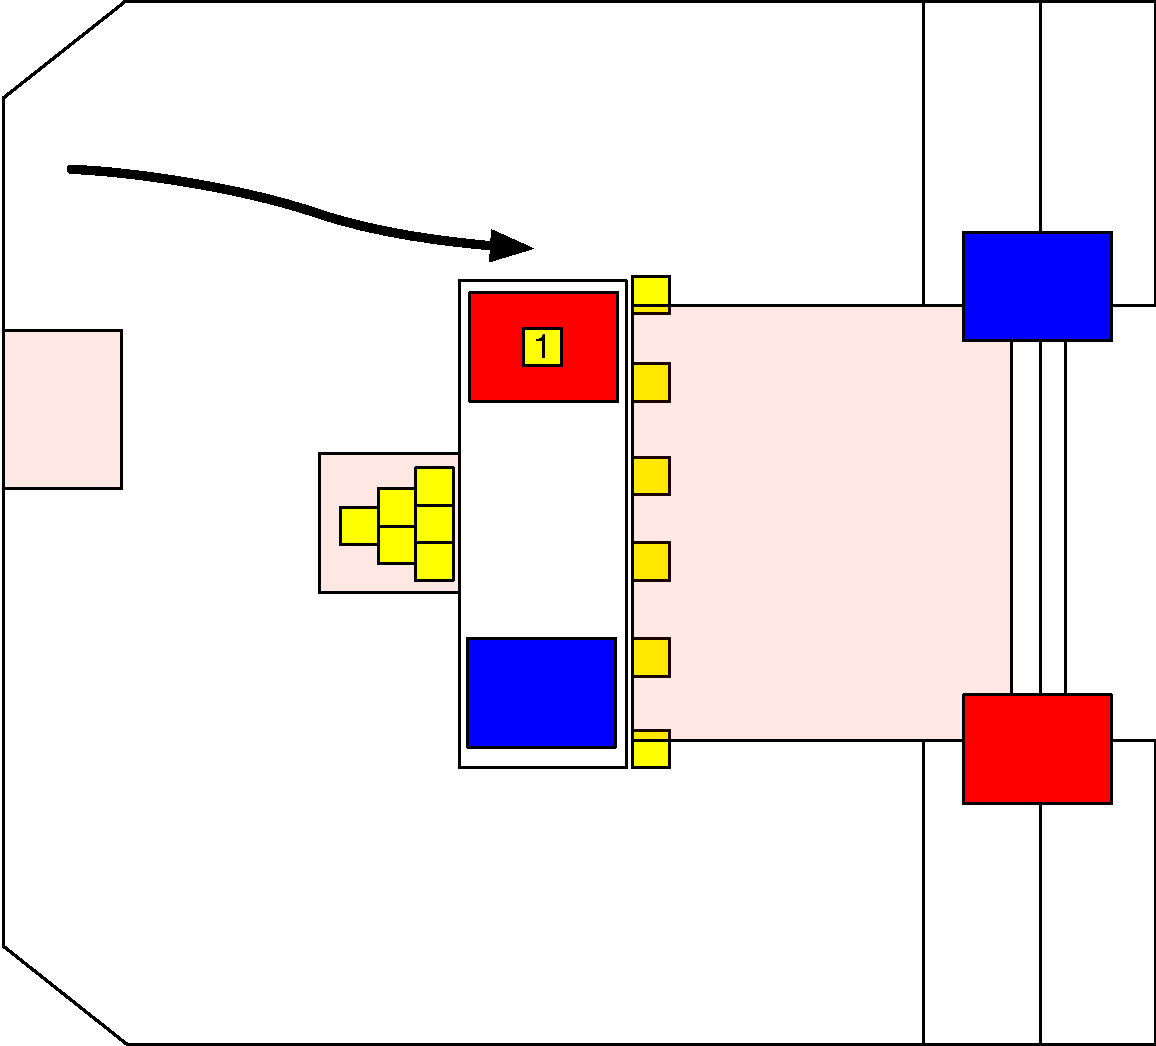
\includegraphics[scale=0.15]{assets/paths/10_LR}
  \end{figure}
  \begin{figure}
   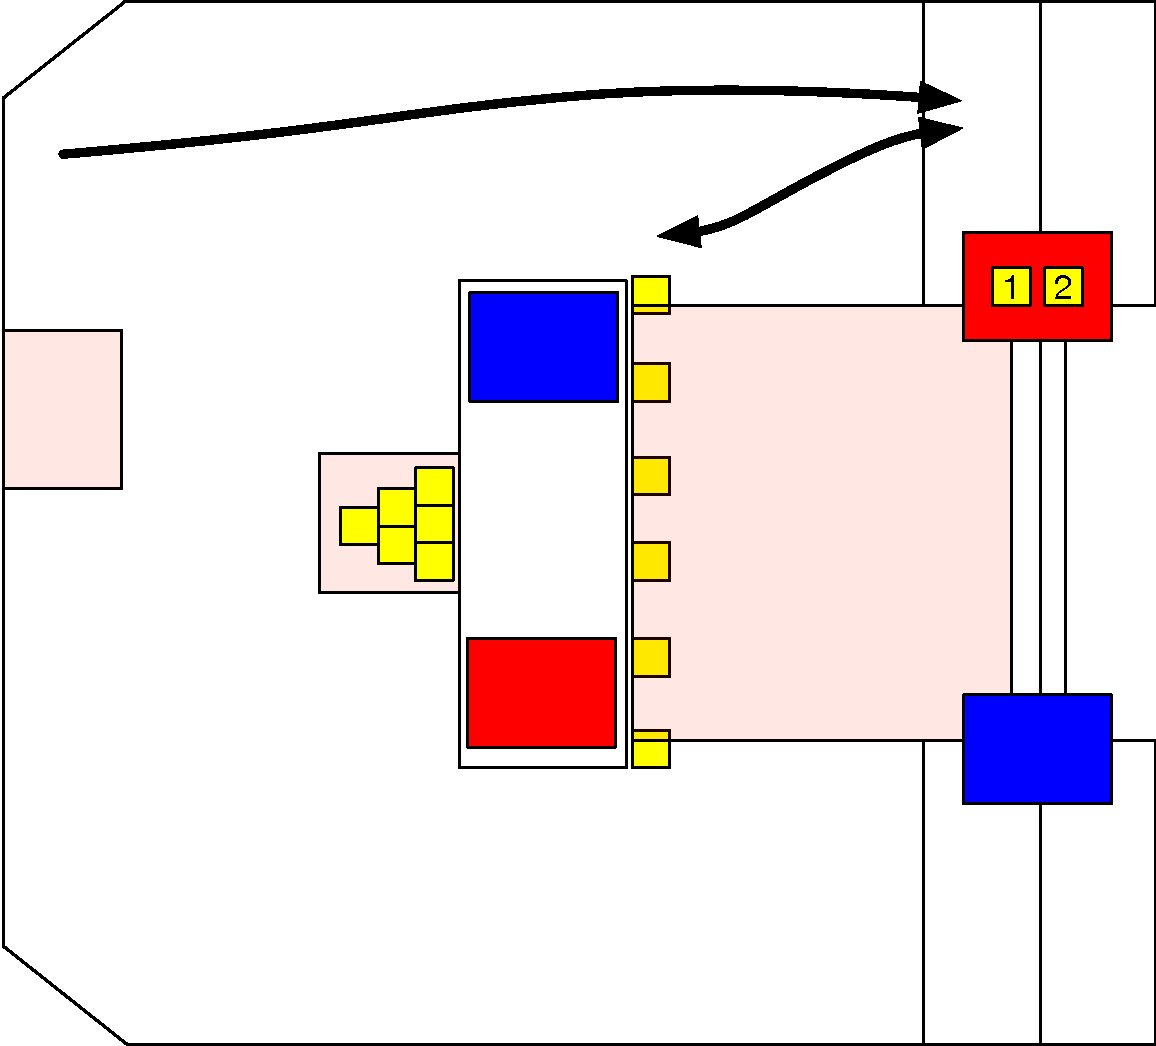
\includegraphics[scale=0.15]{assets/paths/10_RL}
  \end{figure}
  \column{0.5\textwidth}
  \begin{figure}
   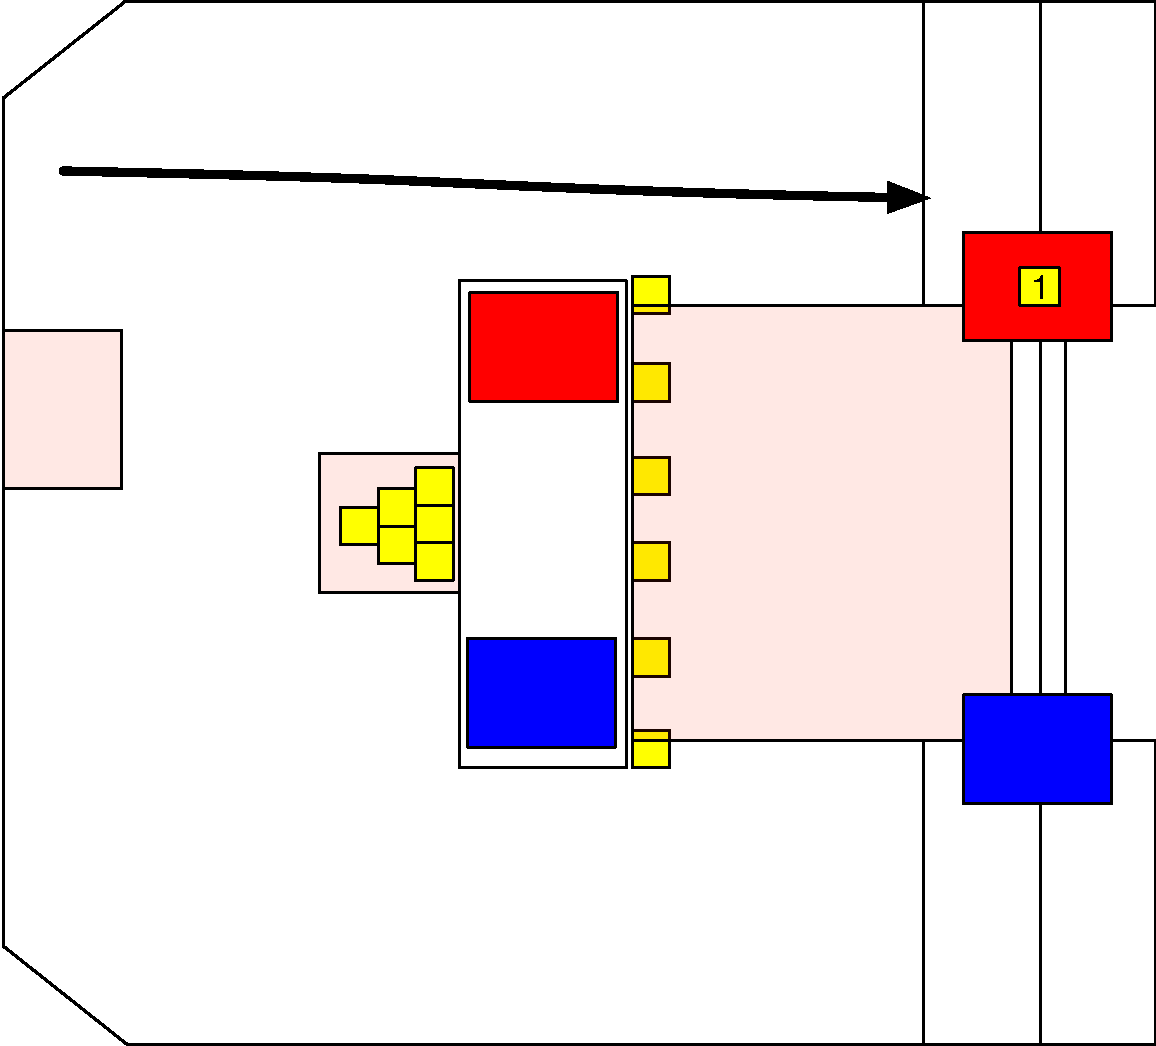
\includegraphics[scale=0.15]{assets/paths/10_LL}
  \end{figure}
  \begin{figure}
   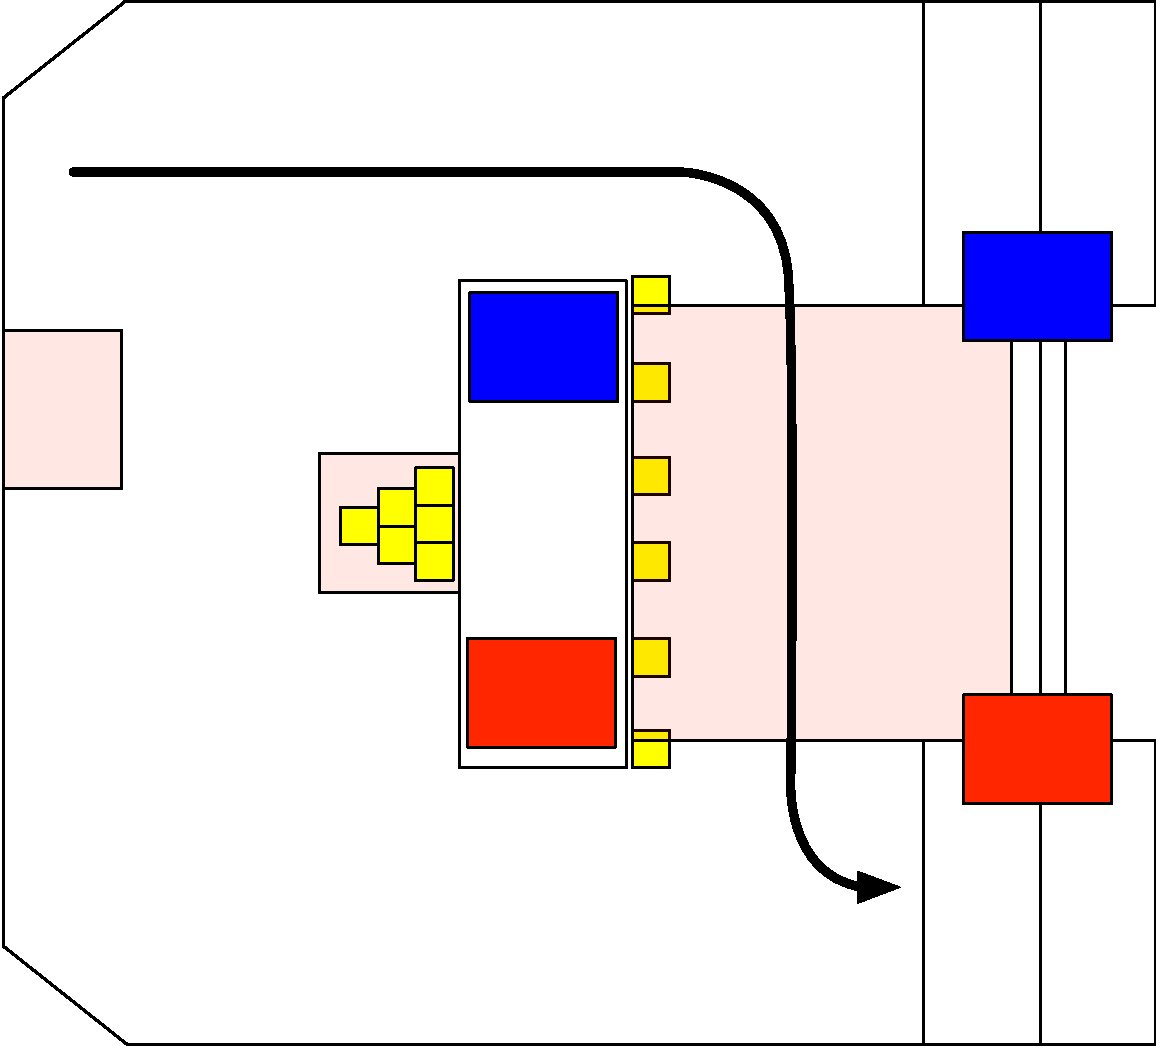
\includegraphics[scale=0.15]{assets/paths/10_RR}
  \end{figure}
 \end{columns}
\end{frame}
%--- Next Frame ---%
\subsection{Switch Priority (11)}

\begin{frame}
 \frametitle{Left Corner Switch Priority \alert{(11)}}
 \begin{columns}
  \column{0.5\textwidth}
  \begin{figure}
   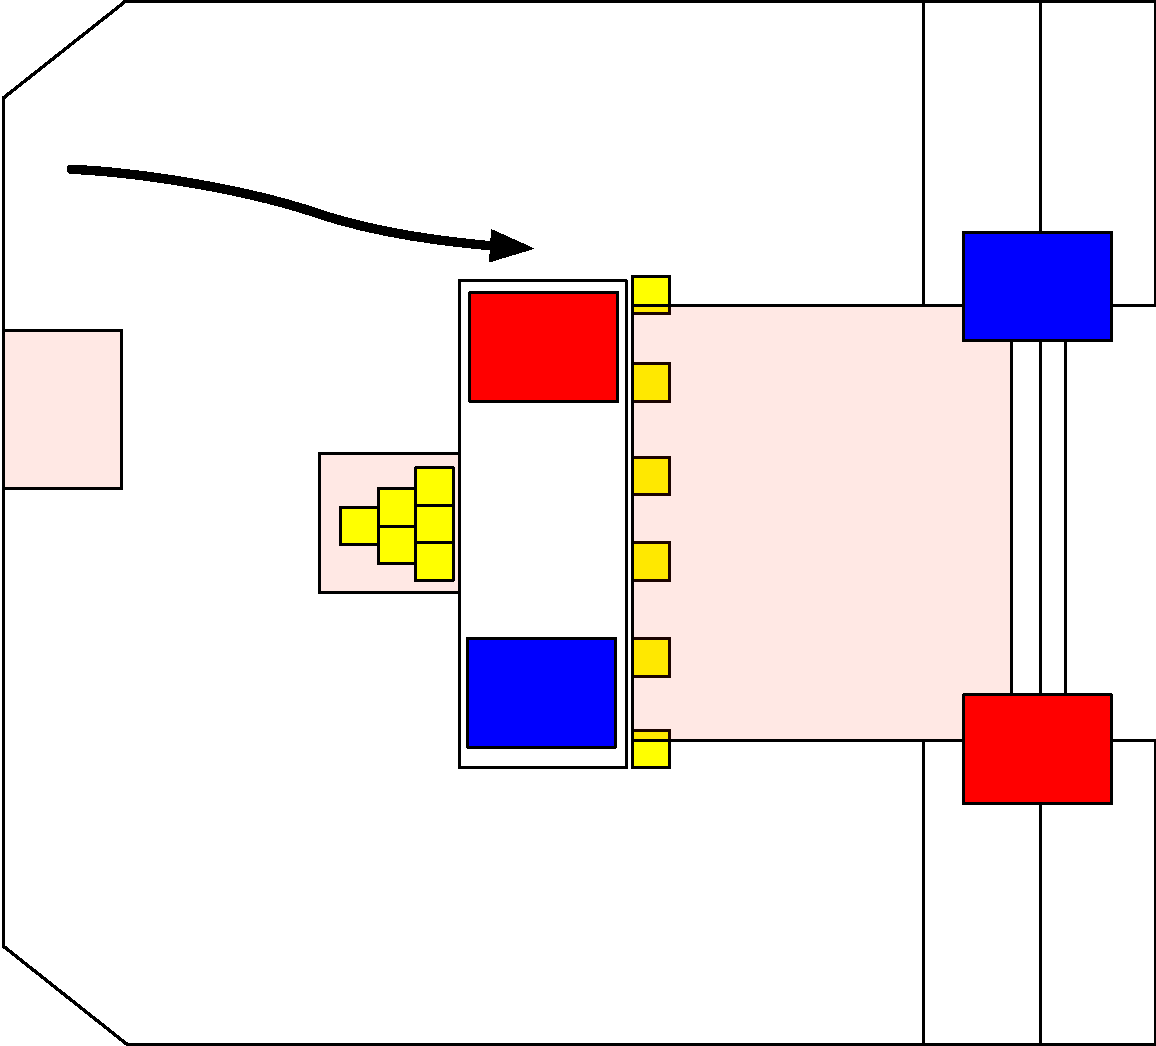
\includegraphics[scale=0.15]{assets/paths/11_LR}
  \end{figure}
  \begin{figure}
   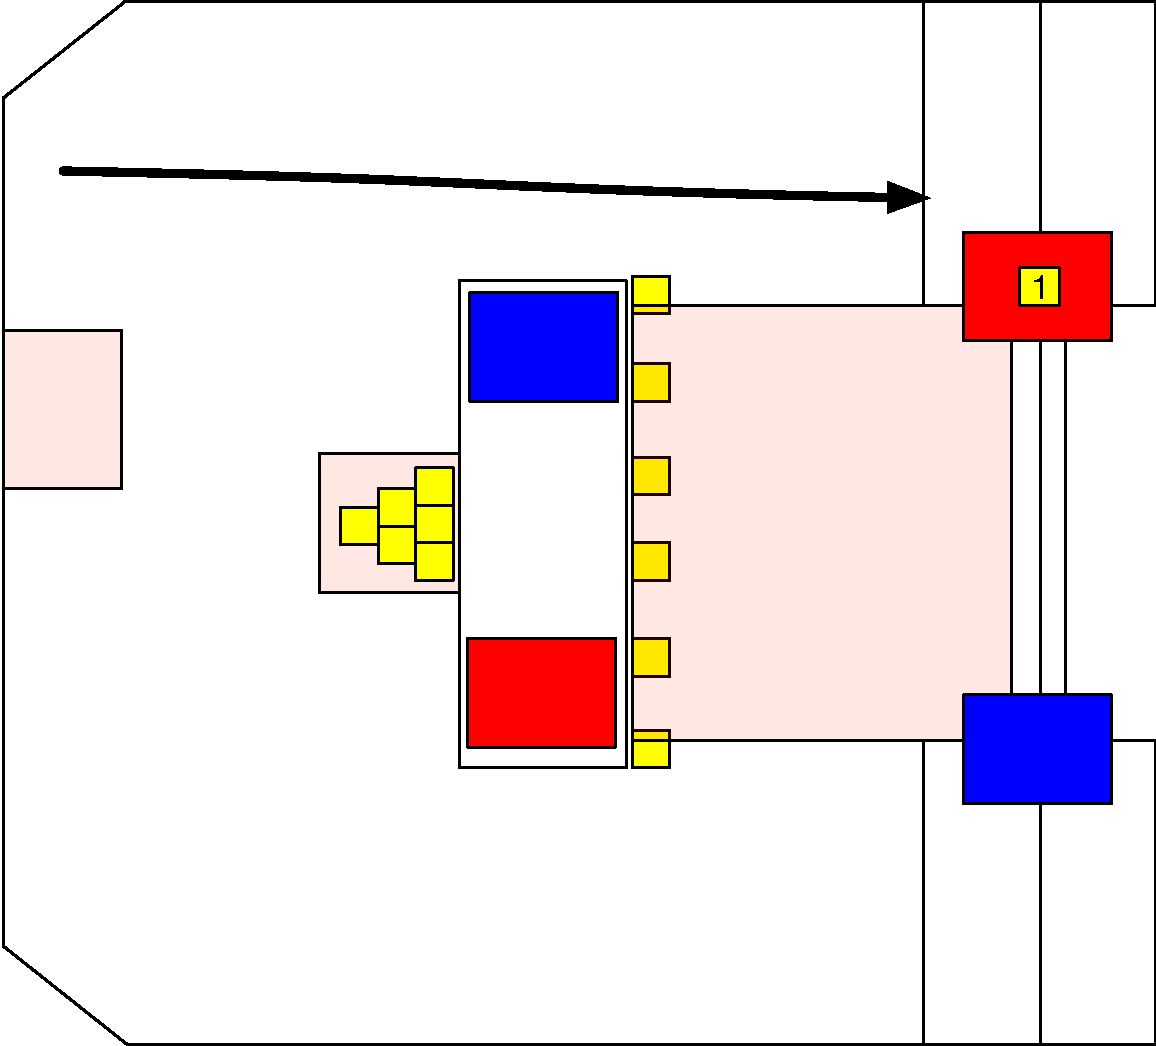
\includegraphics[scale=0.15]{assets/paths/11_RL}
  \end{figure}
  \column{0.5\textwidth}
  \begin{figure}
   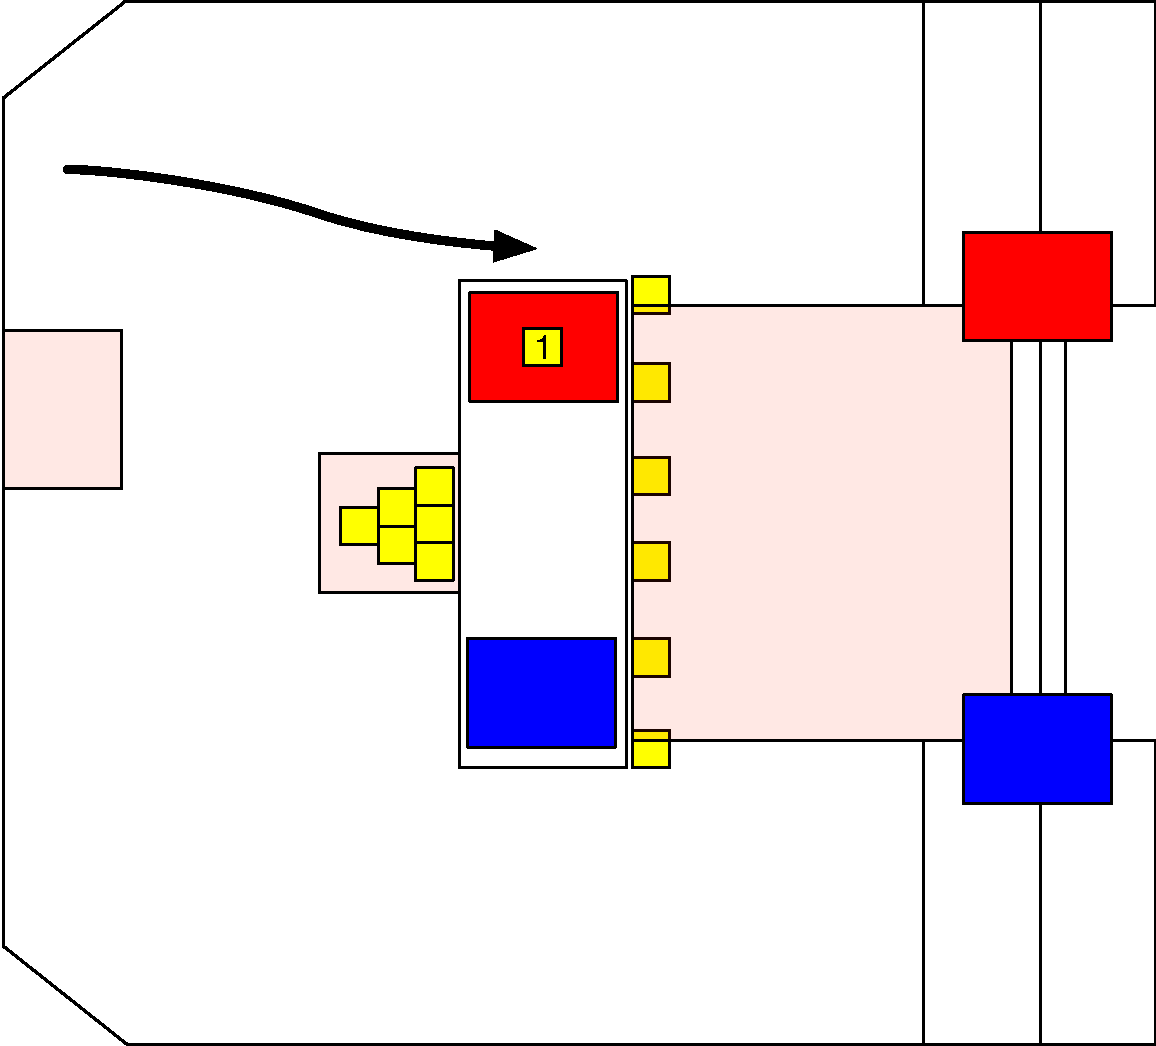
\includegraphics[scale=0.15]{assets/paths/11_LL}
  \end{figure}
  \begin{figure}
   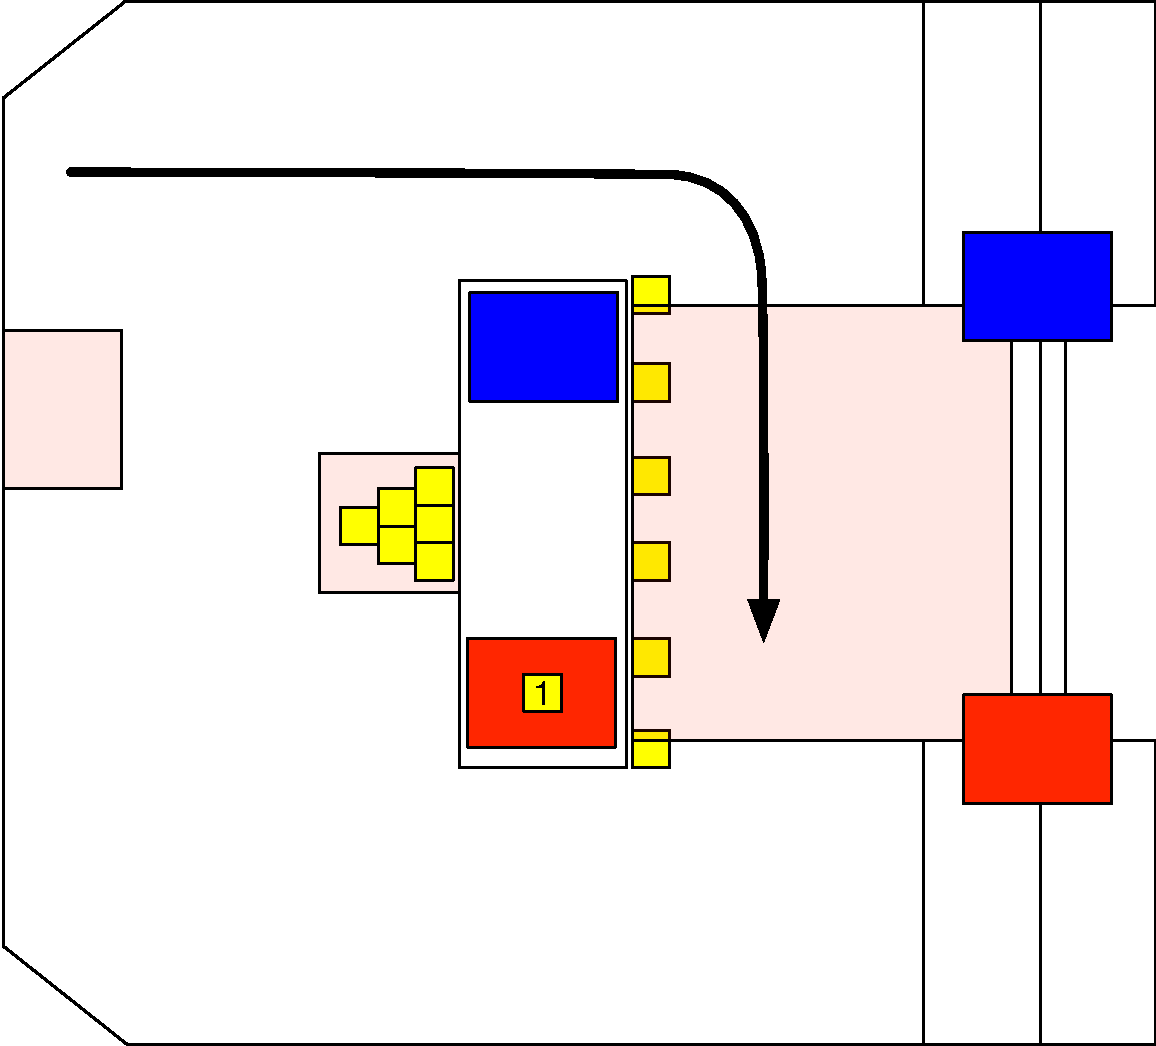
\includegraphics[scale=0.15]{assets/paths/11_RR}
  \end{figure}
 \end{columns}
\end{frame}
%--- Next Frame ---%
\subsection{Switch Priority, Opposite Scale Backup (12)}

\begin{frame}
 \frametitle{Left Corner Switch Priority, Opposite Scale Backup \alert{(12)}}
 \begin{columns}
  \column{0.5\textwidth}
  \begin{figure}
   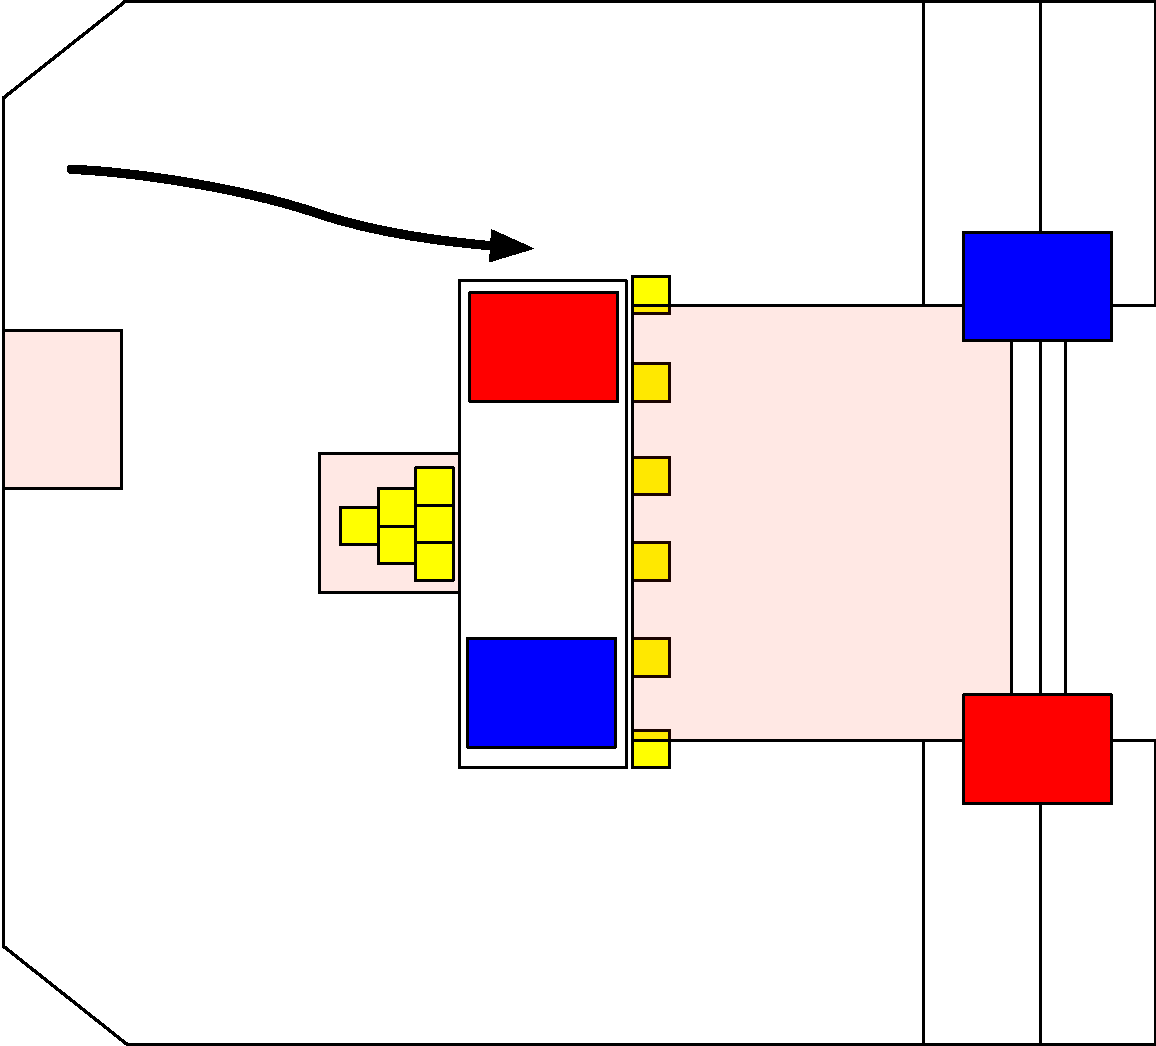
\includegraphics[scale=0.15]{assets/paths/12_LR}
  \end{figure}
  \begin{figure}
   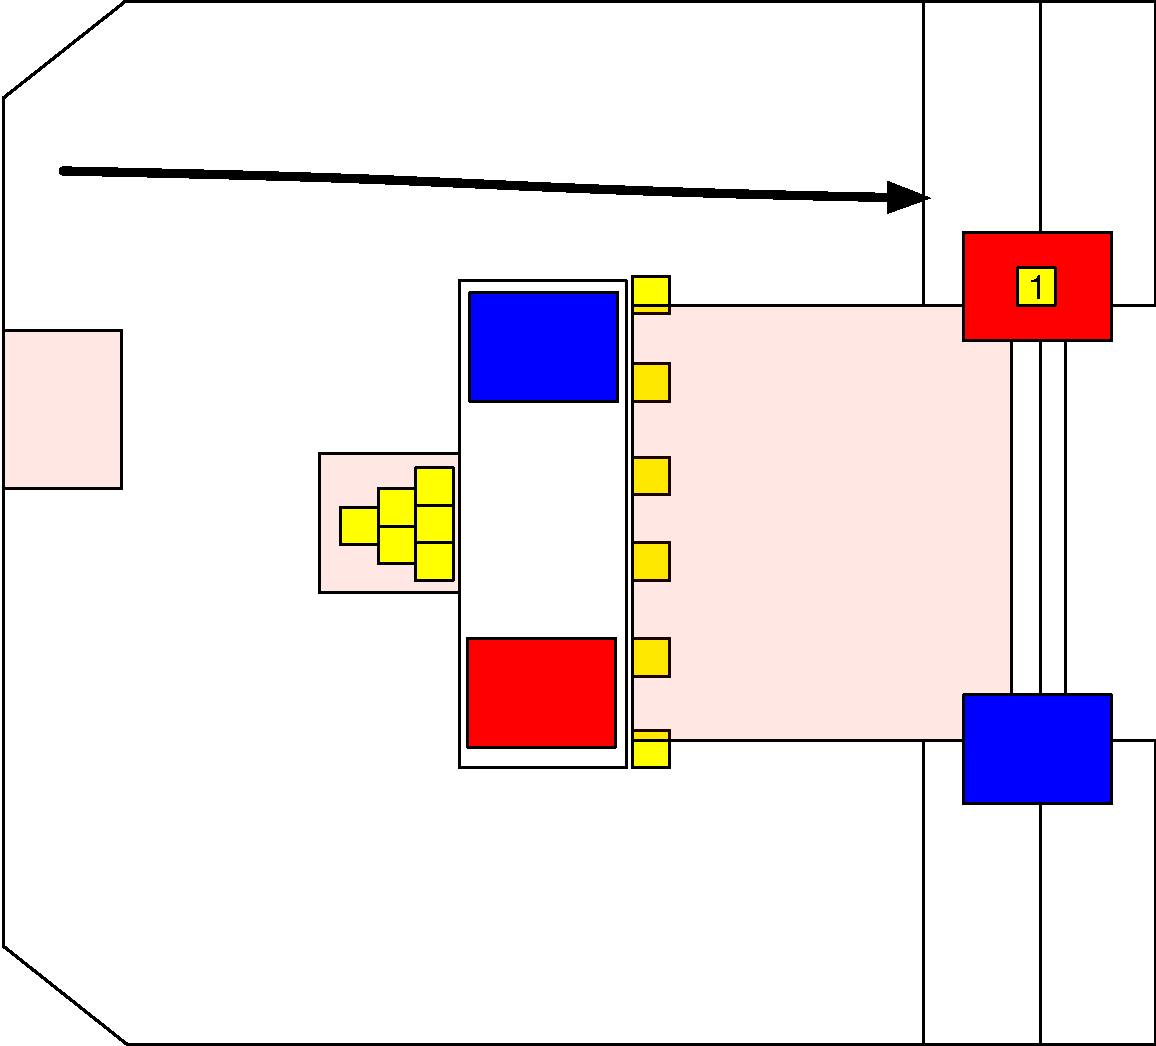
\includegraphics[scale=0.15]{assets/paths/12_RL}
  \end{figure}
  \column{0.5\textwidth}
  \begin{figure}
   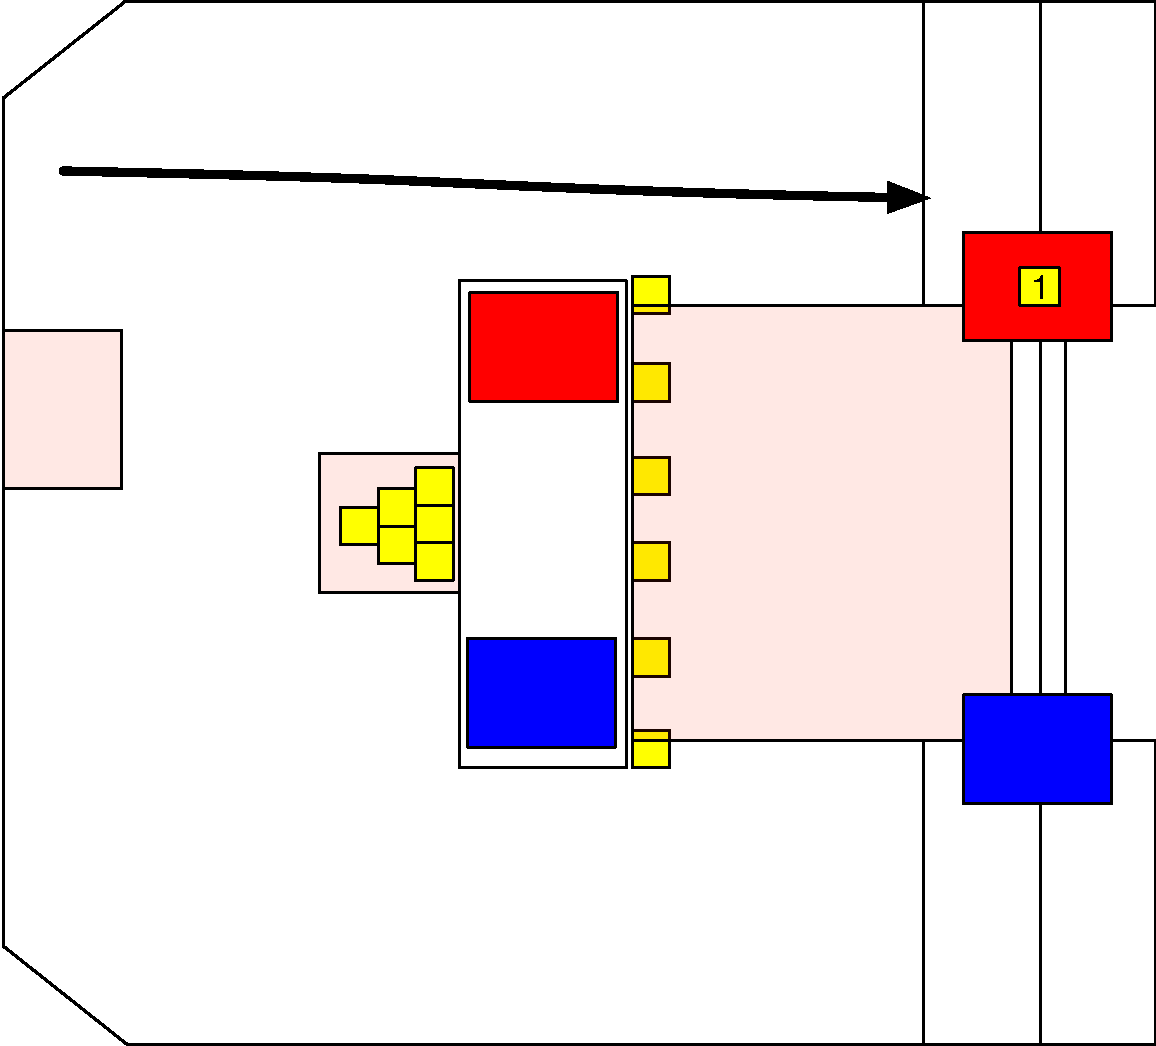
\includegraphics[scale=0.15]{assets/paths/12_LL}
  \end{figure}
  \begin{figure}
   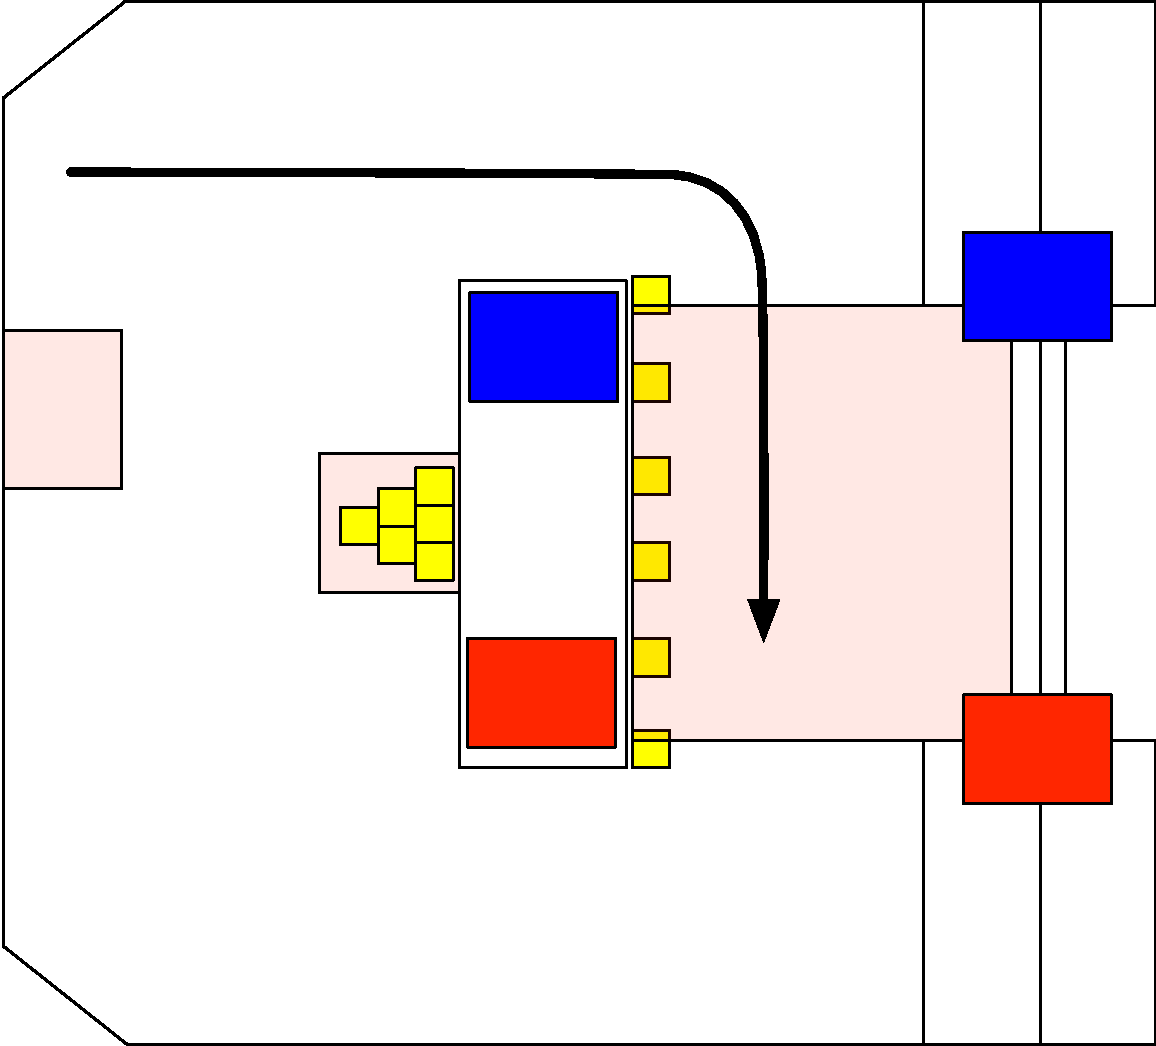
\includegraphics[scale=0.15]{assets/paths/12_RR}
  \end{figure}
 \end{columns}
\end{frame}
%--- Next Frame ---%

\section{Center}
\subsection{Switch Priority (20)}

\begin{frame}
 \frametitle{Center Switch Priority \alert{(20)}}
 \begin{columns}
  \column{0.5\textwidth}
  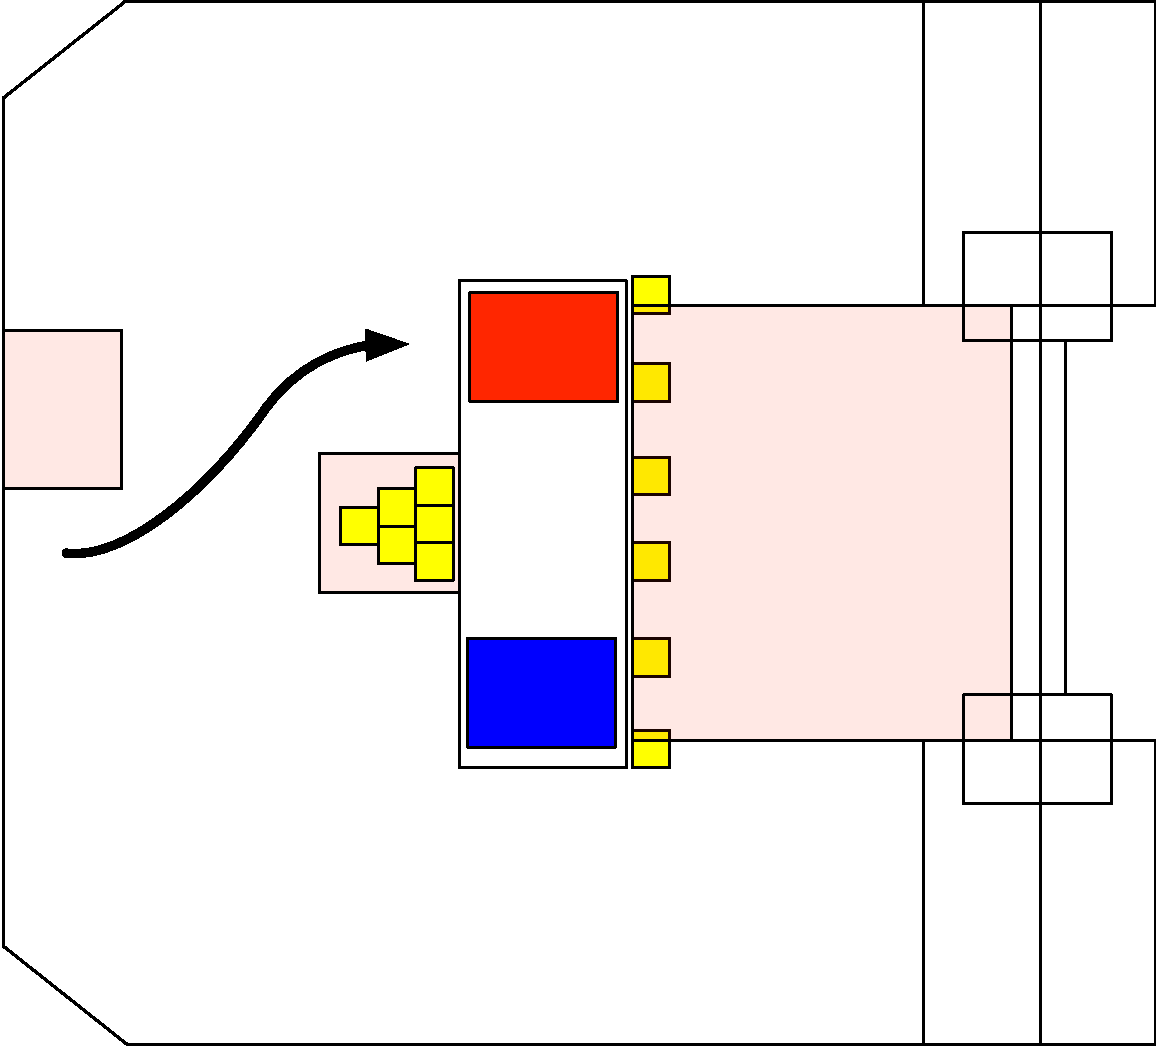
\includegraphics[scale=0.25]{assets/paths/20_LX}
  \column{0.5\textwidth}
  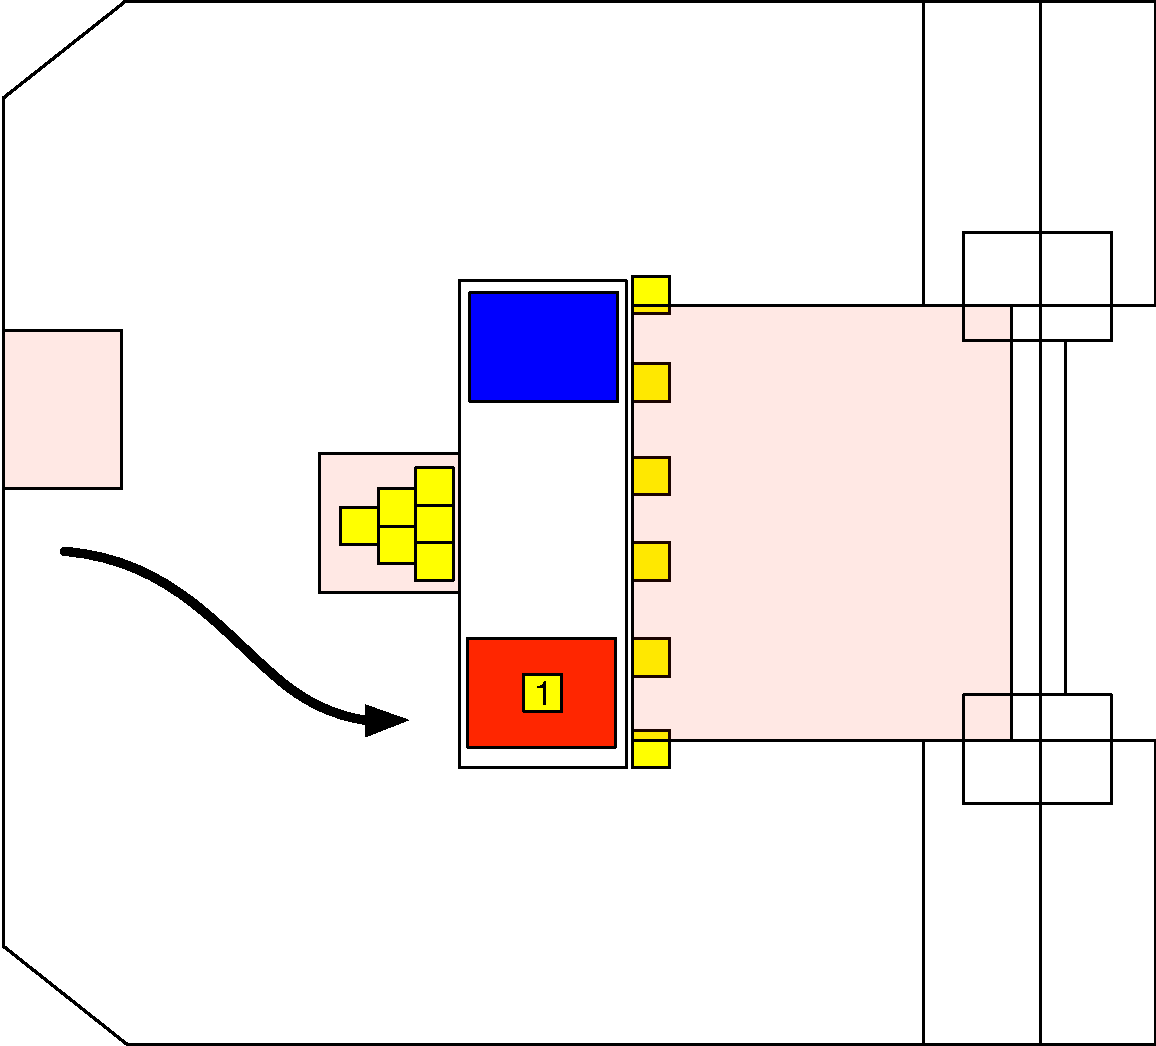
\includegraphics[scale=0.25]{assets/paths/20_RX}
 \end{columns}
\end{frame}
%--- Next Frame ---%
\section{Right Corner}
\subsection{Scale Priority (30)}

\begin{frame}
 \frametitle{Right Corner Scale Priority \alert{(30)}}
 \begin{columns}
  \column{0.5\textwidth}
  \begin{figure}
   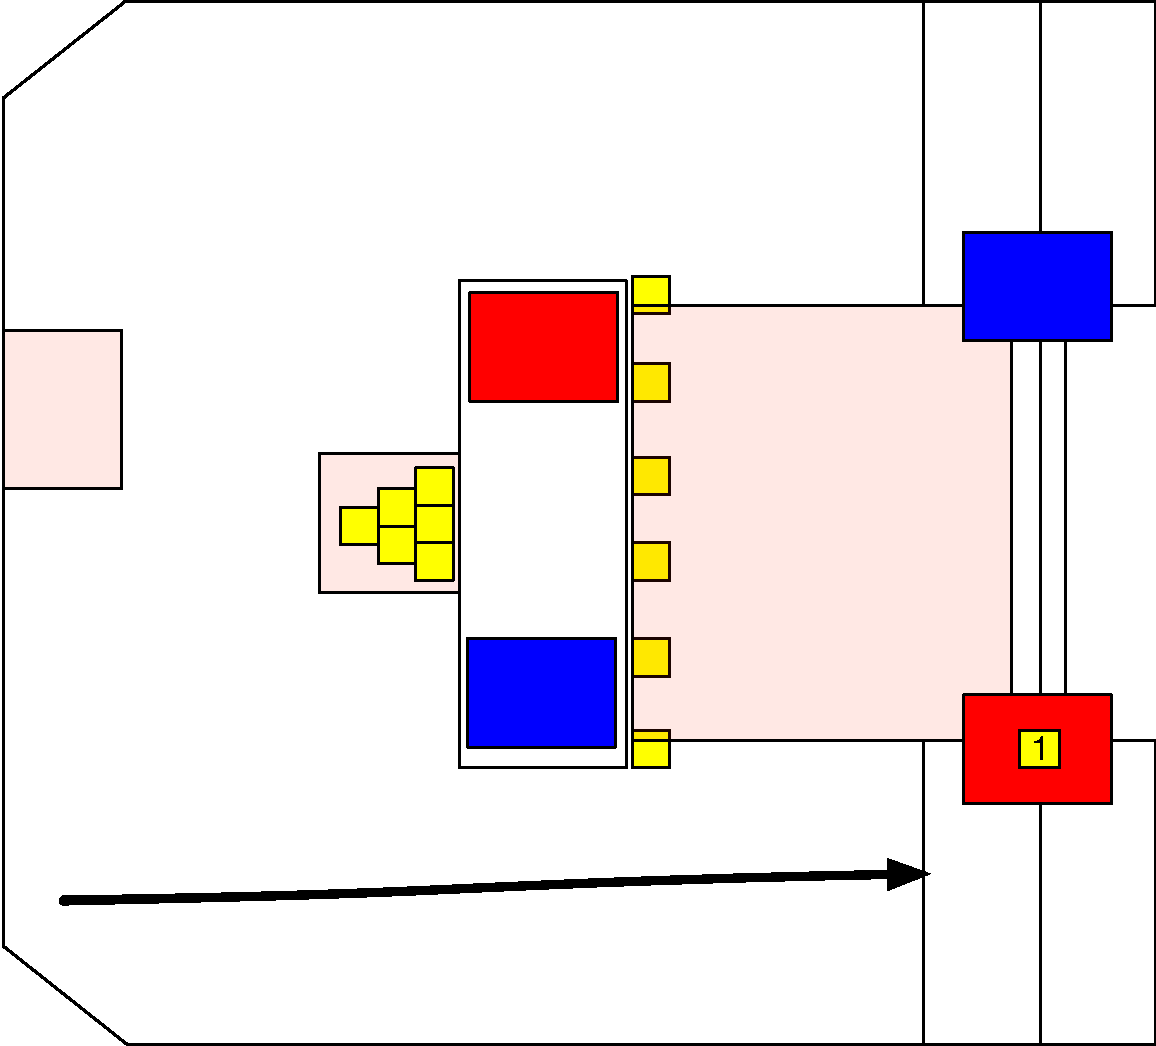
\includegraphics[scale=0.15]{assets/paths/30_LR}
  \end{figure}
  \begin{figure}
   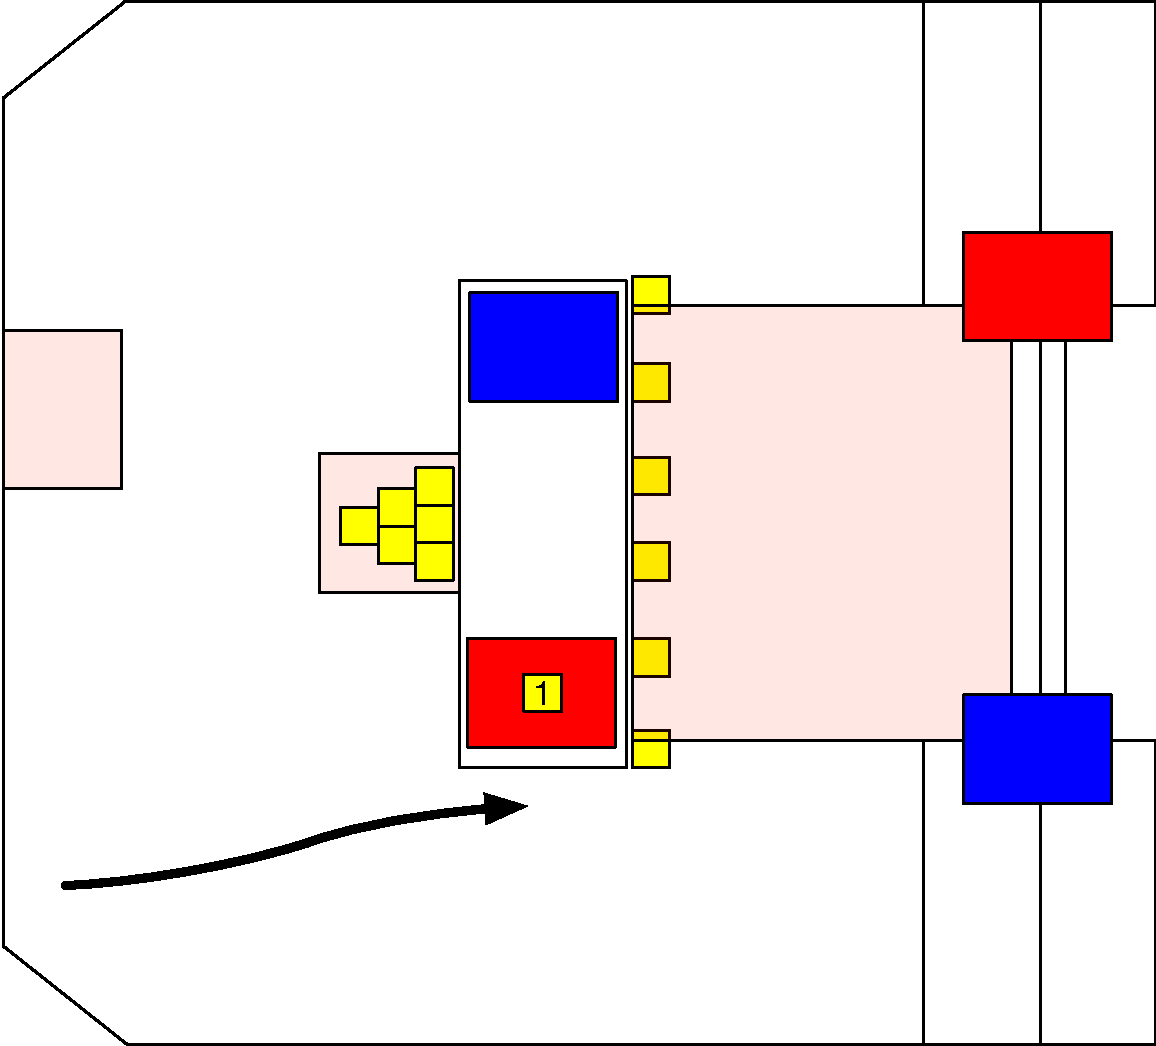
\includegraphics[scale=0.15]{assets/paths/30_RL}
  \end{figure}
  \column{0.5\textwidth}
  \begin{figure}
   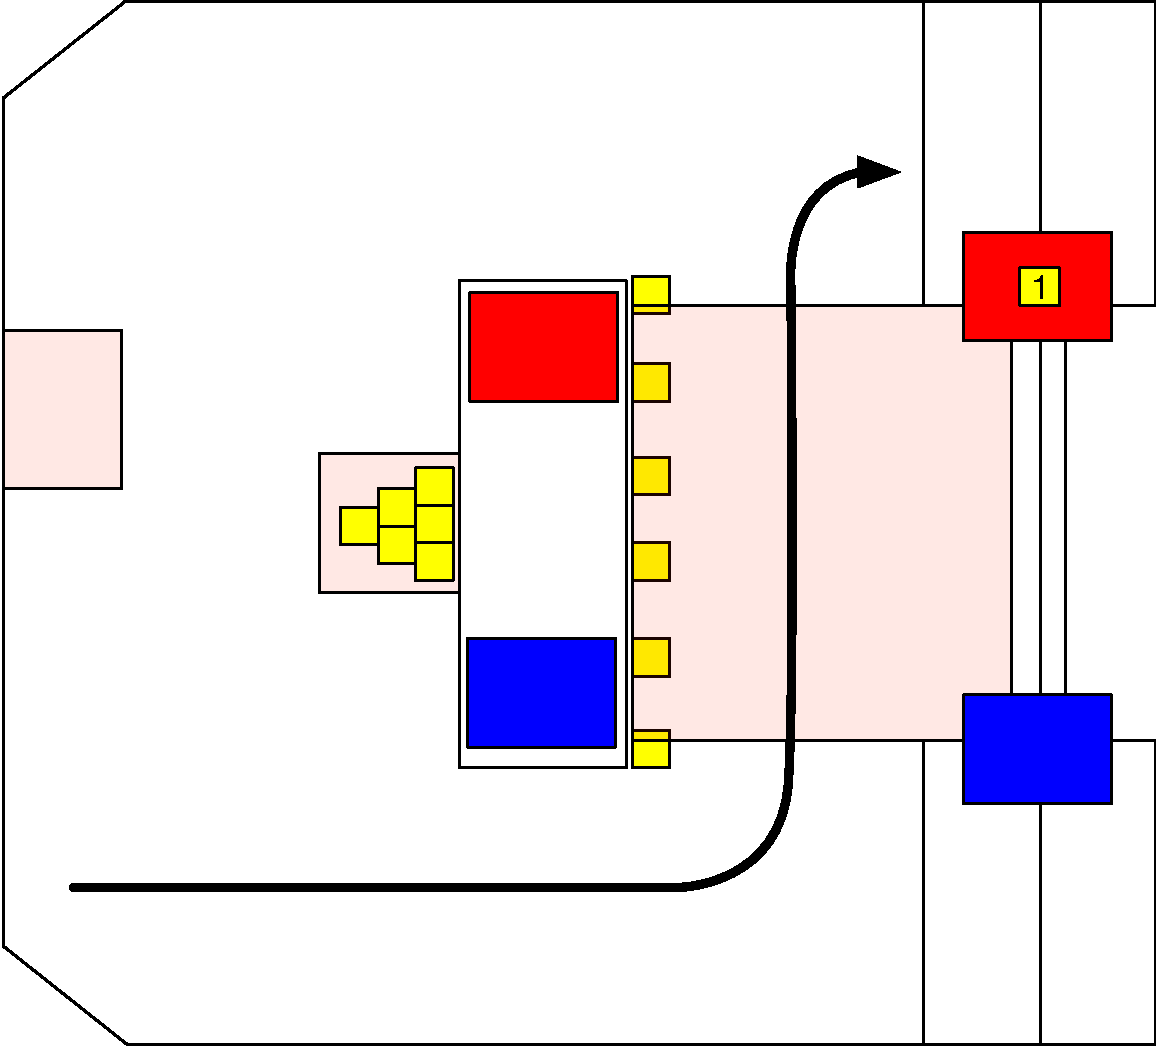
\includegraphics[scale=0.15]{assets/paths/30_LL}
  \end{figure}
  \begin{figure}
   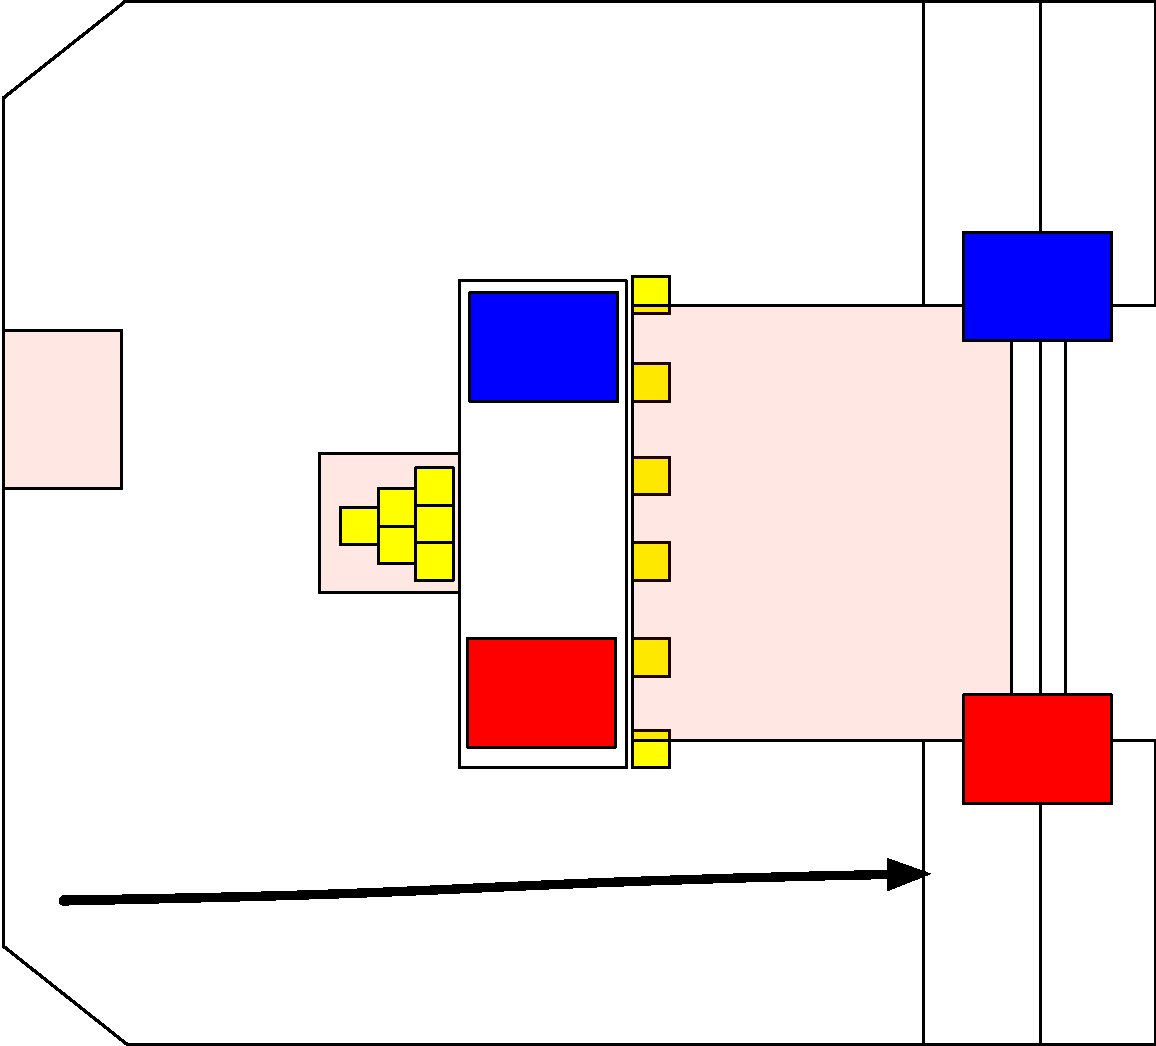
\includegraphics[scale=0.15]{assets/paths/30_RR}
  \end{figure}
 \end{columns}
\end{frame}
%--- Next Frame ---%
\subsection{Switch Priority (31)}

\begin{frame}
 \frametitle{Right Corner Switch Priority \alert{(31)}}
 \begin{columns}
  \column{0.5\textwidth}
  \begin{figure}
   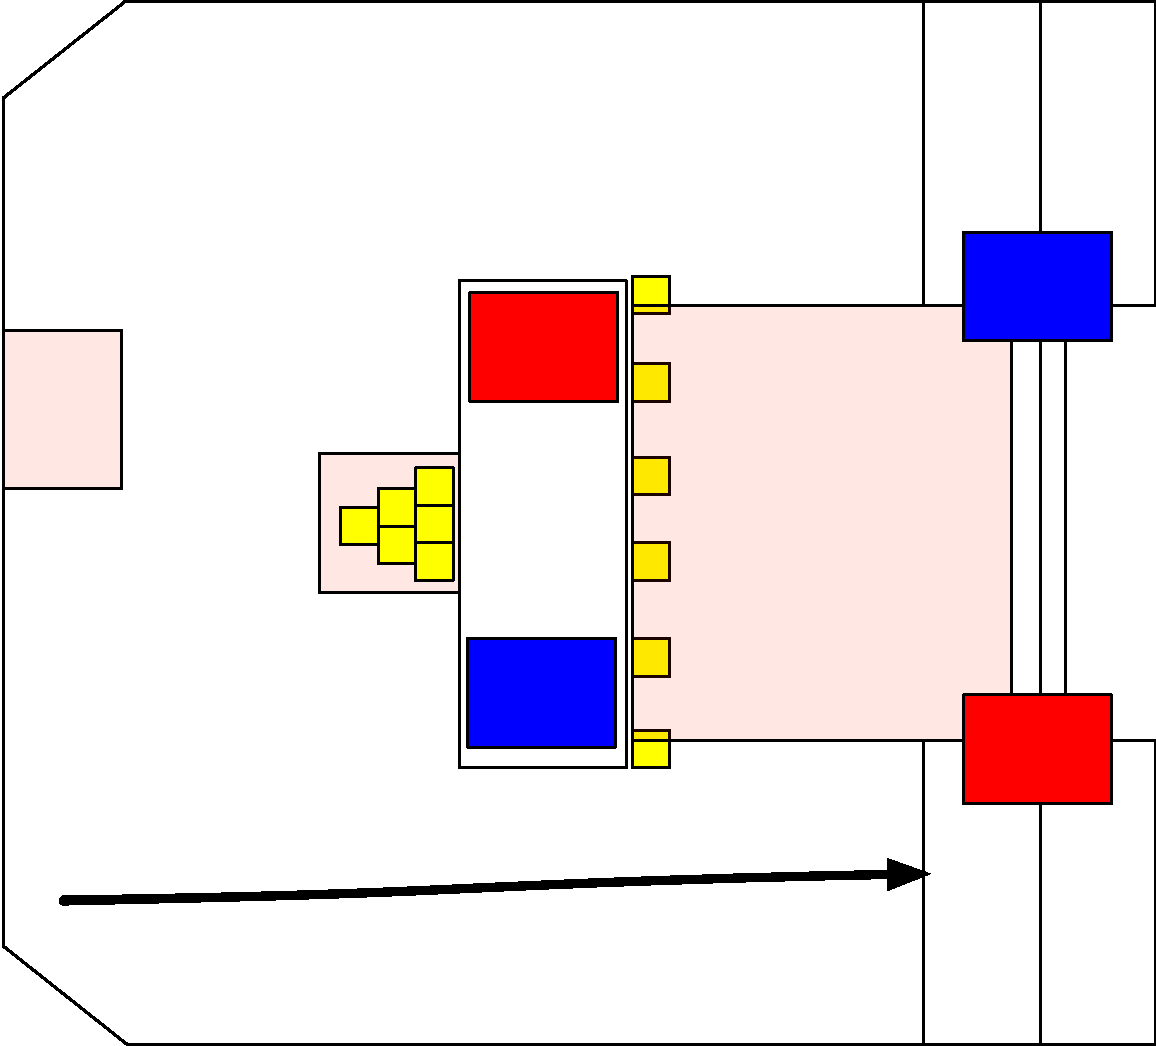
\includegraphics[scale=0.15]{assets/paths/31_LR}
  \end{figure}
  \begin{figure}
   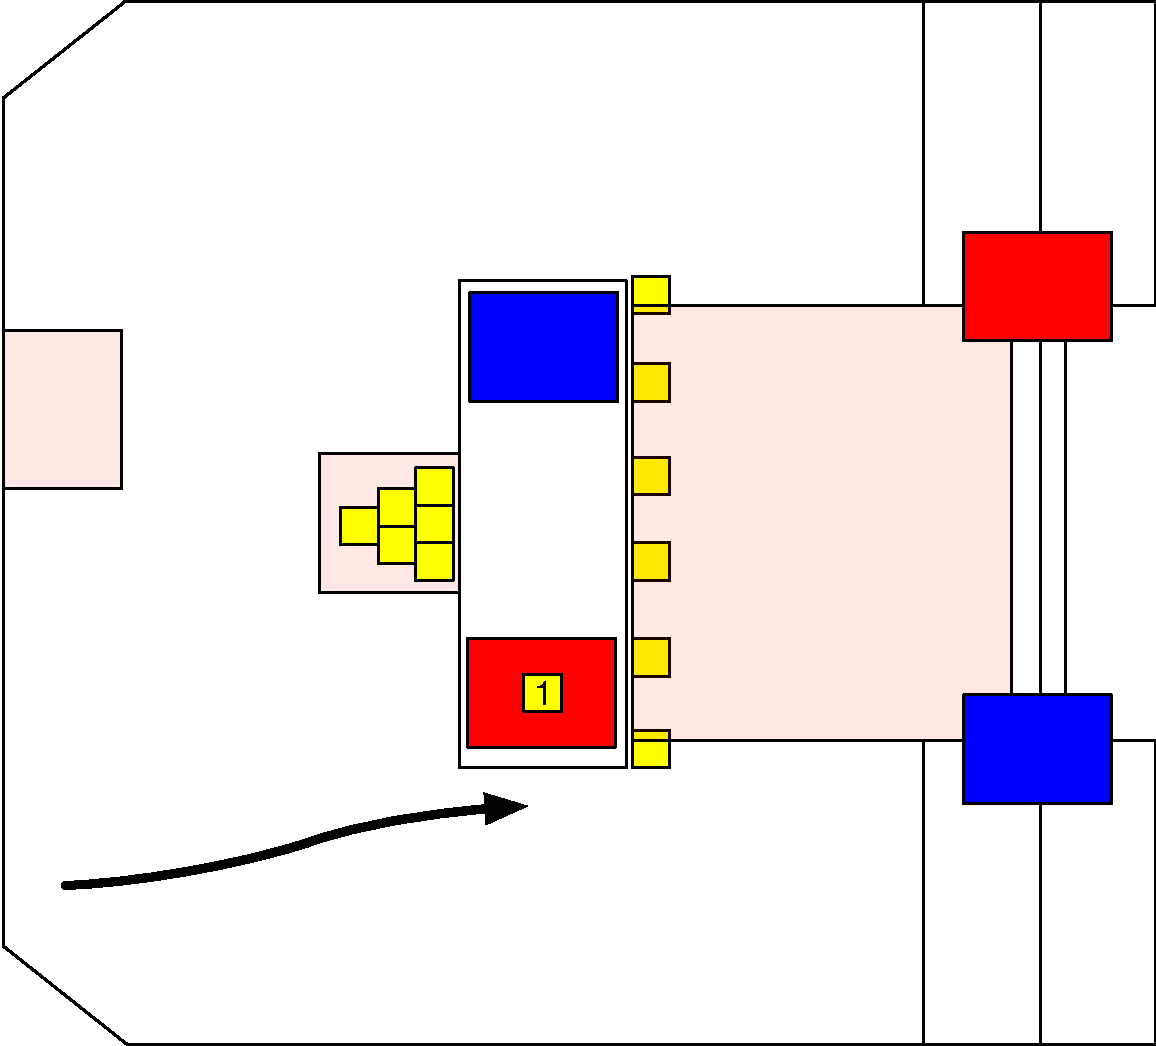
\includegraphics[scale=0.15]{assets/paths/31_RL}
  \end{figure}
  \column{0.5\textwidth}
  \begin{figure}
   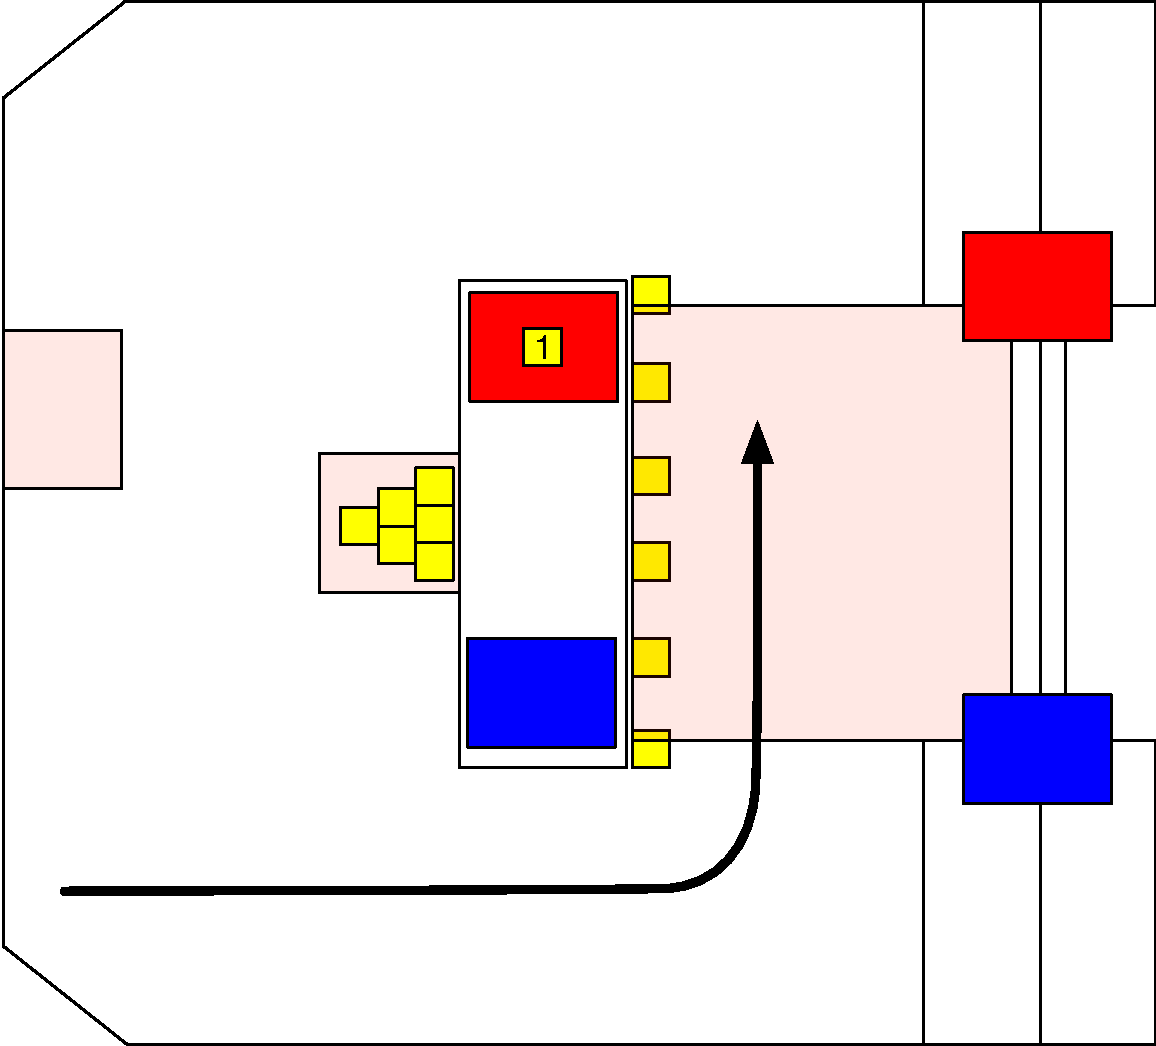
\includegraphics[scale=0.15]{assets/paths/31_LL}
  \end{figure}
  \begin{figure}
   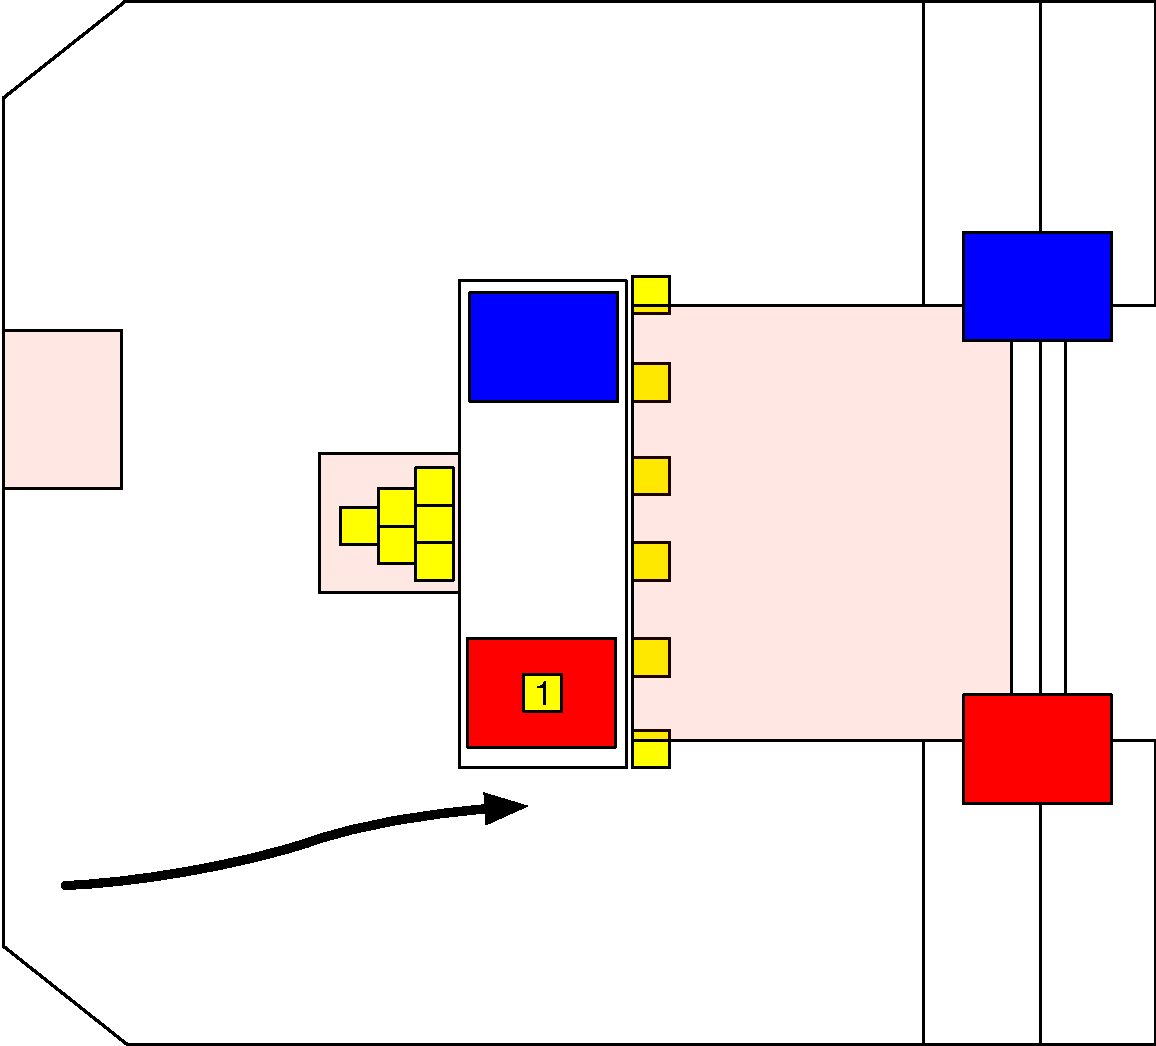
\includegraphics[scale=0.15]{assets/paths/31_RR}
  \end{figure}
 \end{columns}
\end{frame}
%--- Next Frame ---%
\subsection{Switch Priority, Opposite Scale Backup (32)}

\begin{frame}
 \frametitle{Right Corner Switch Priority, Opposite Scale Backup \alert{(32)}}
 \begin{columns}
  \column{0.5\textwidth}
  \begin{figure}
   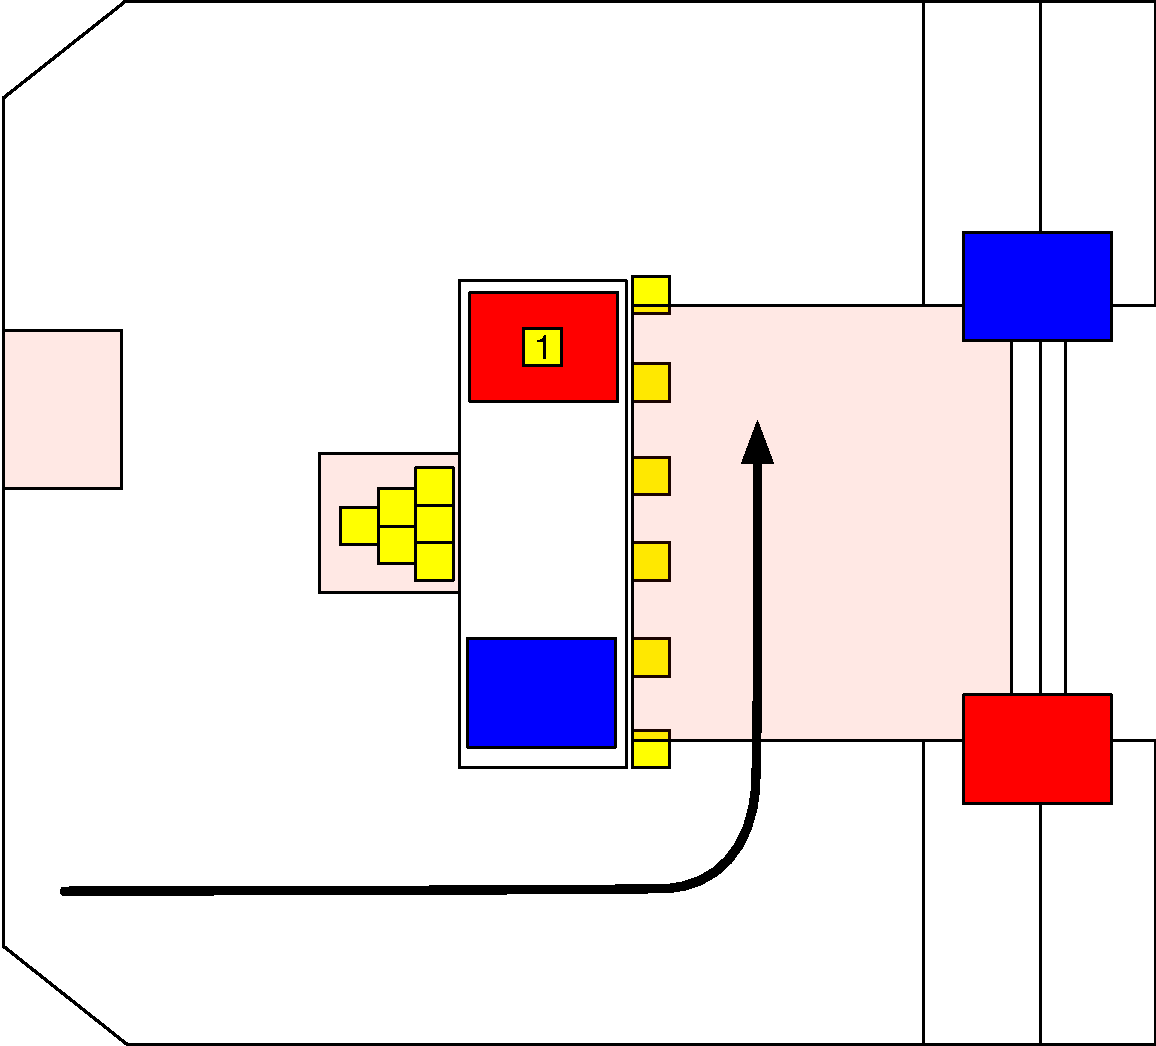
\includegraphics[scale=0.15]{assets/paths/32_LR}
  \end{figure}
  \begin{figure}
   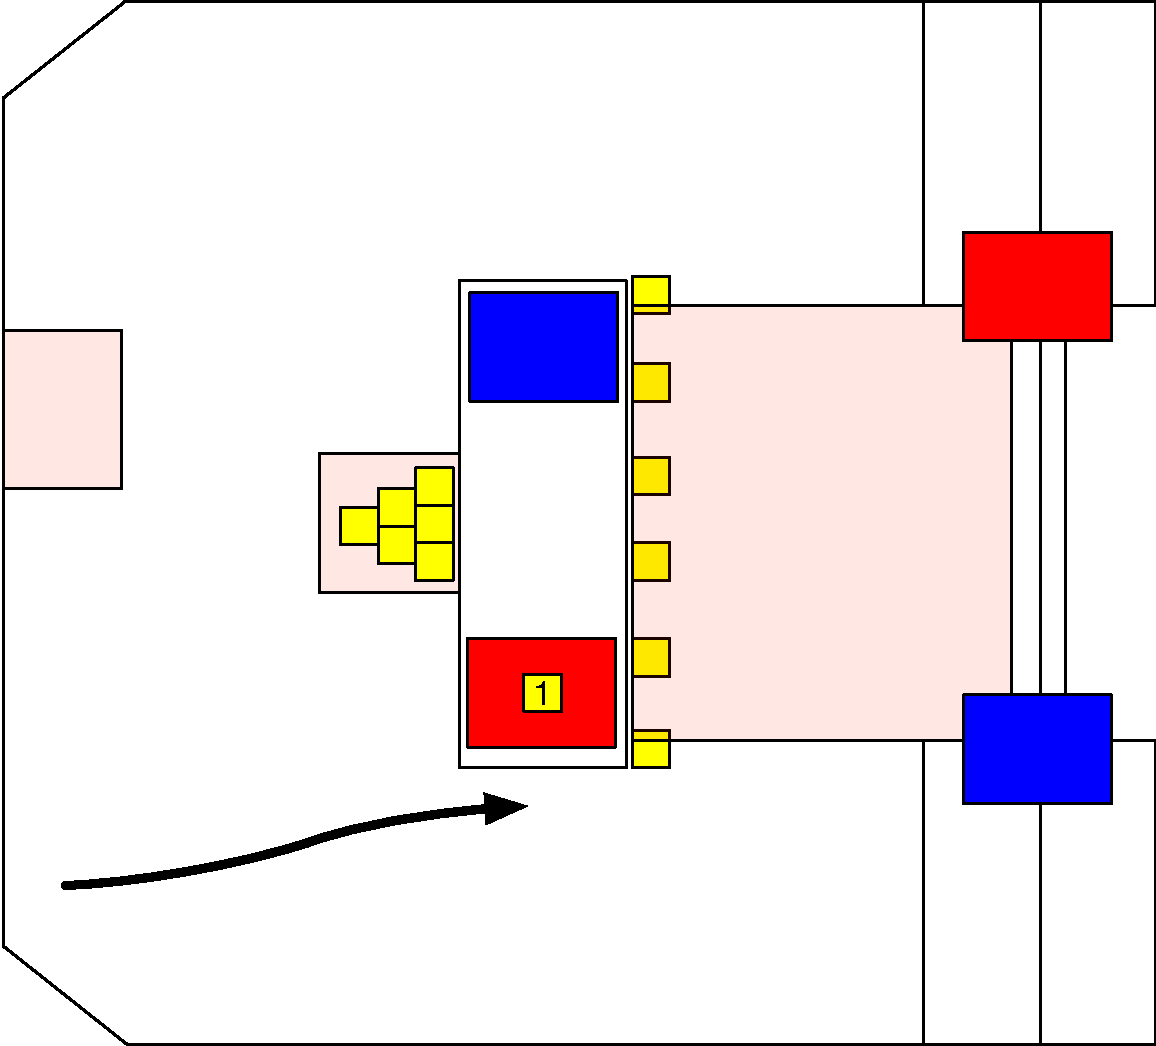
\includegraphics[scale=0.15]{assets/paths/32_RL}
  \end{figure}
  \column{0.5\textwidth}
  \begin{figure}
   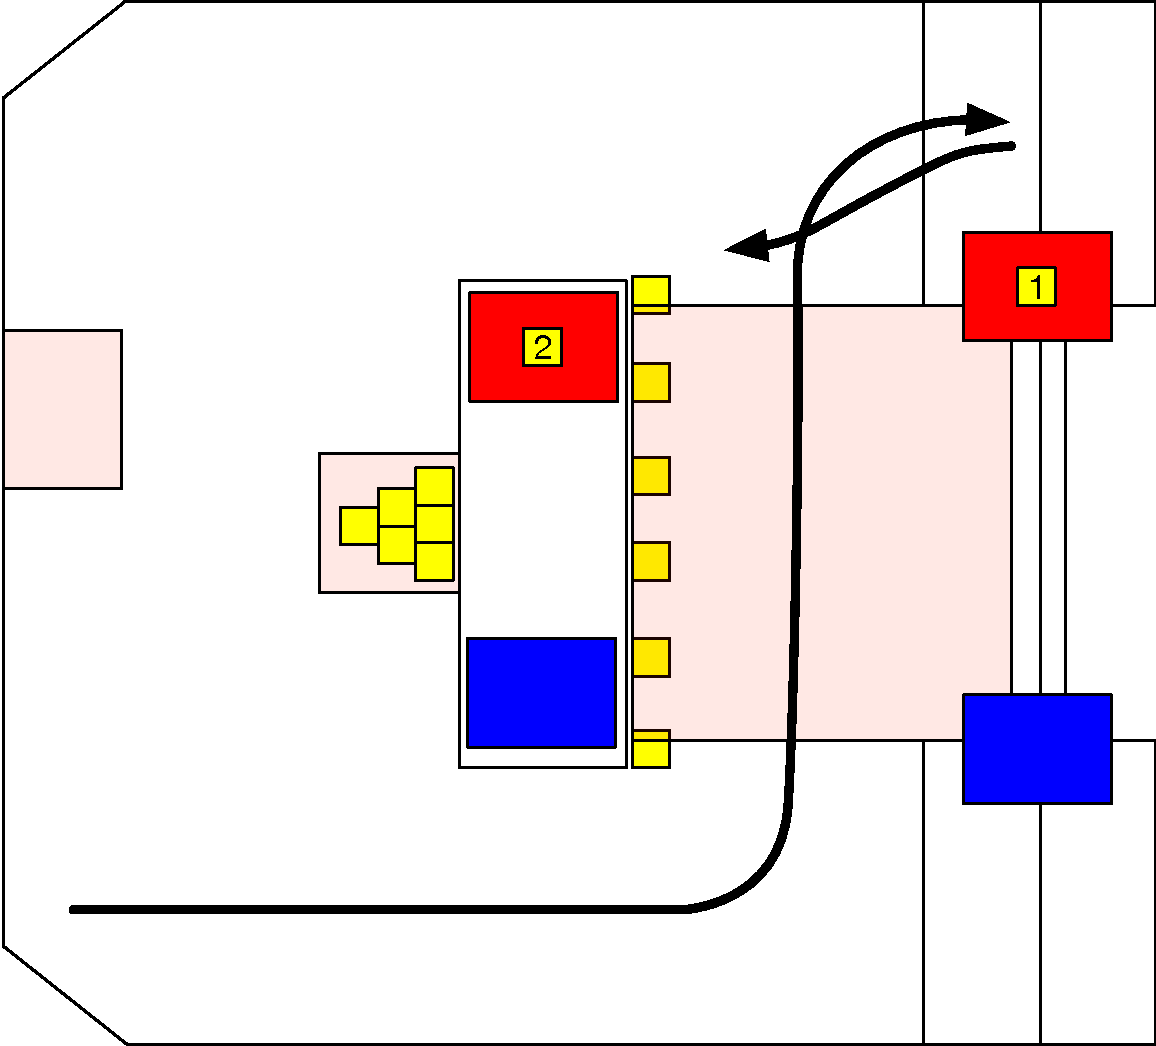
\includegraphics[scale=0.15]{assets/paths/32_LL}
  \end{figure}
  \begin{figure}
   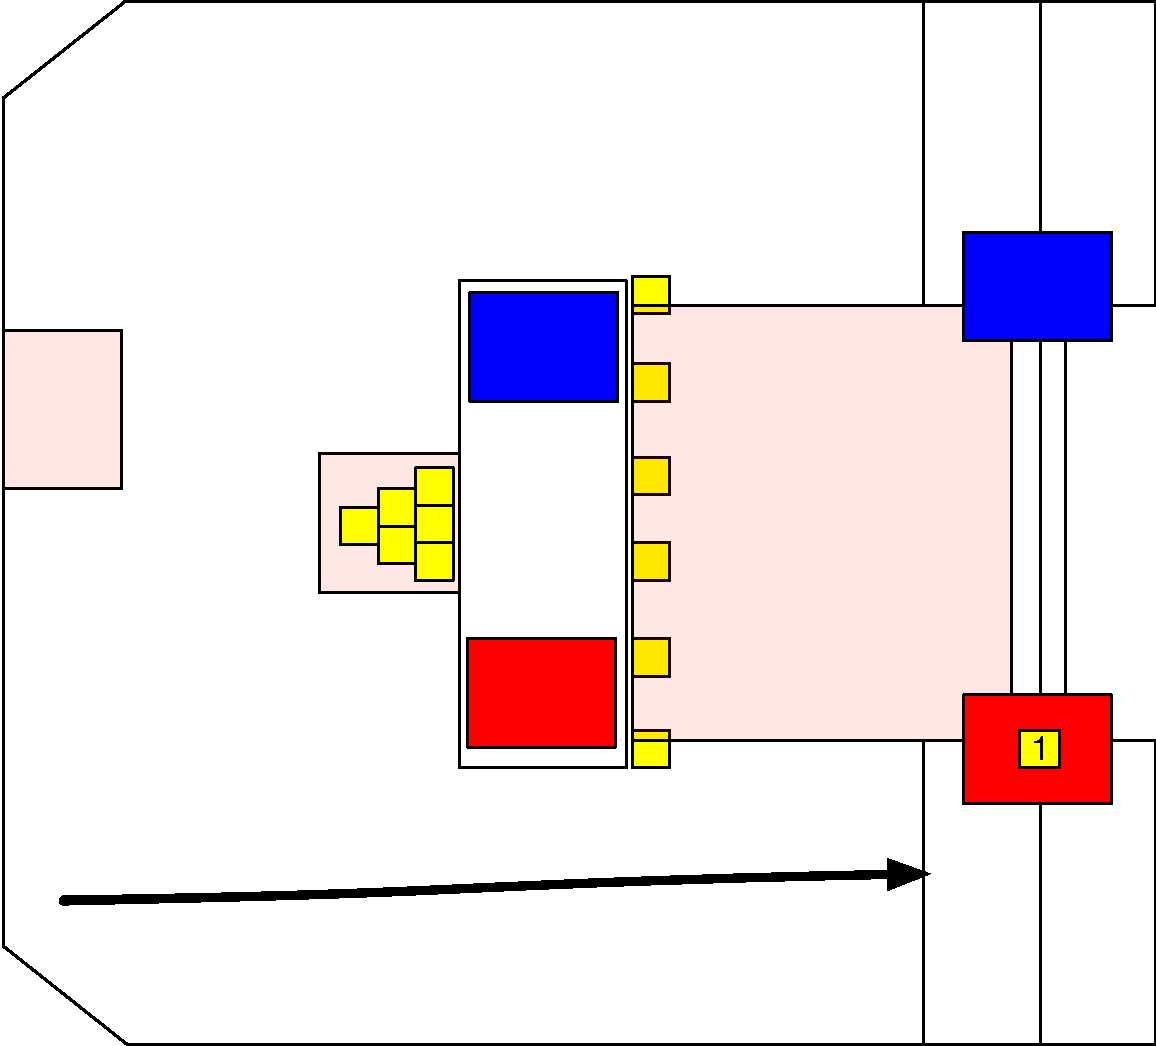
\includegraphics[scale=0.15]{assets/paths/32_RR}
  \end{figure}
 \end{columns}
\end{frame}

\section{Blank Templates}

\begin{frame}
 \frametitle{Blank Templates}
 \begin{columns}
  \column{0.5\textwidth}
  \begin{figure}
   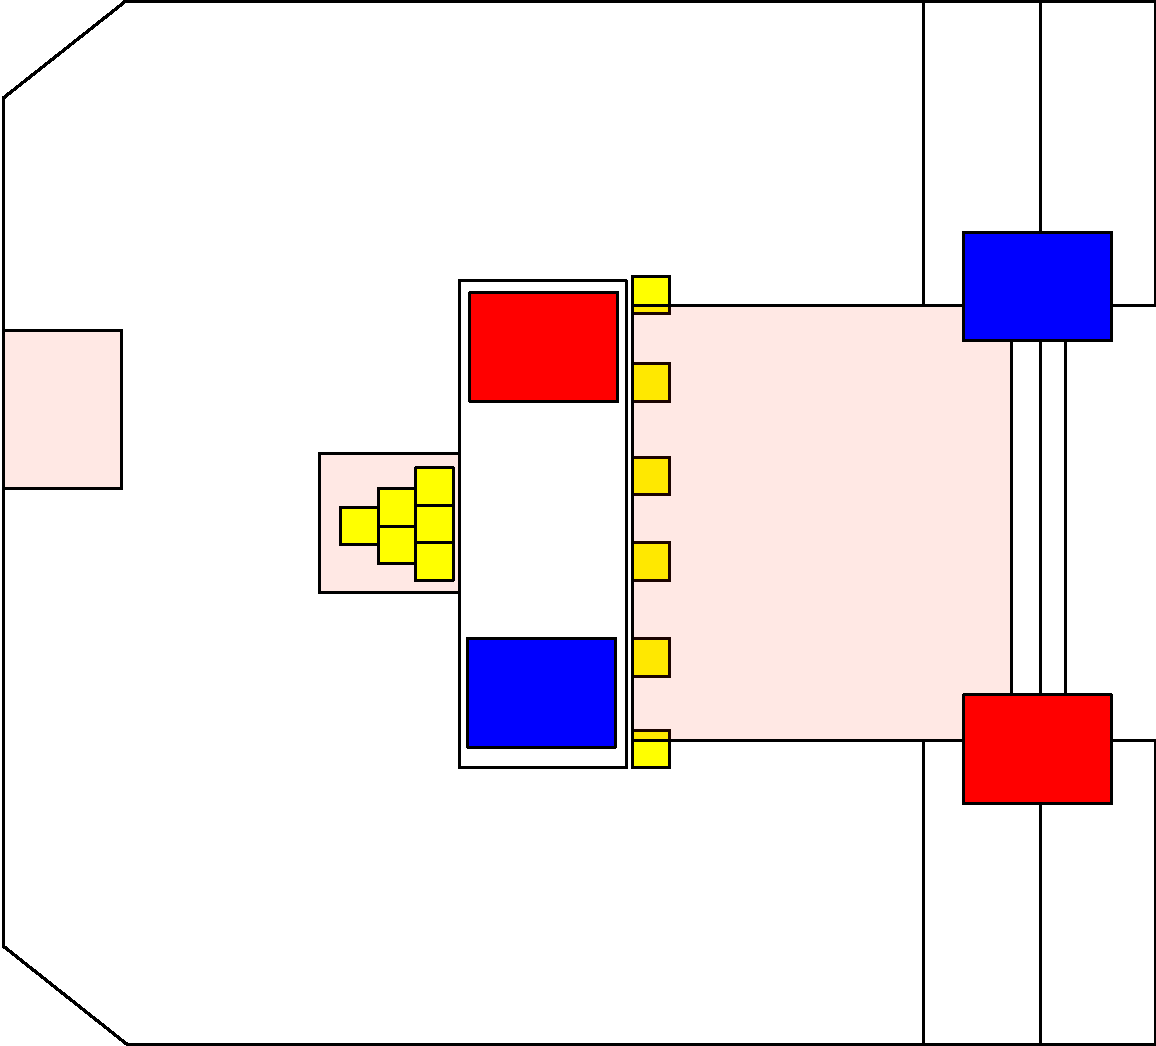
\includegraphics[scale=0.15]{assets/paths/BLANK_LR}
  \end{figure}
  \begin{figure}
   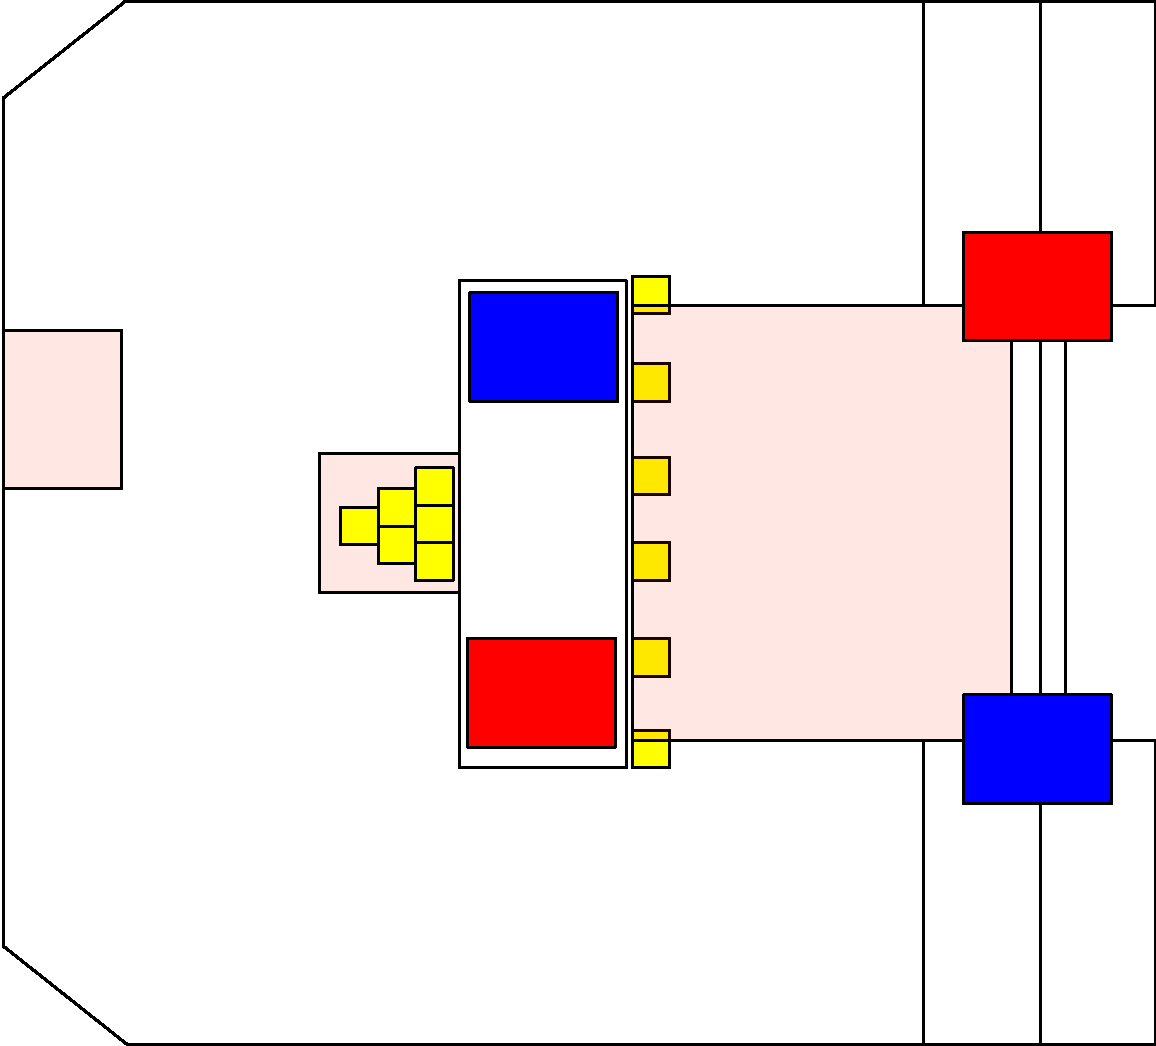
\includegraphics[scale=0.15]{assets/paths/BLANK_RL}
  \end{figure}
  \column{0.5\textwidth}
  \begin{figure}
   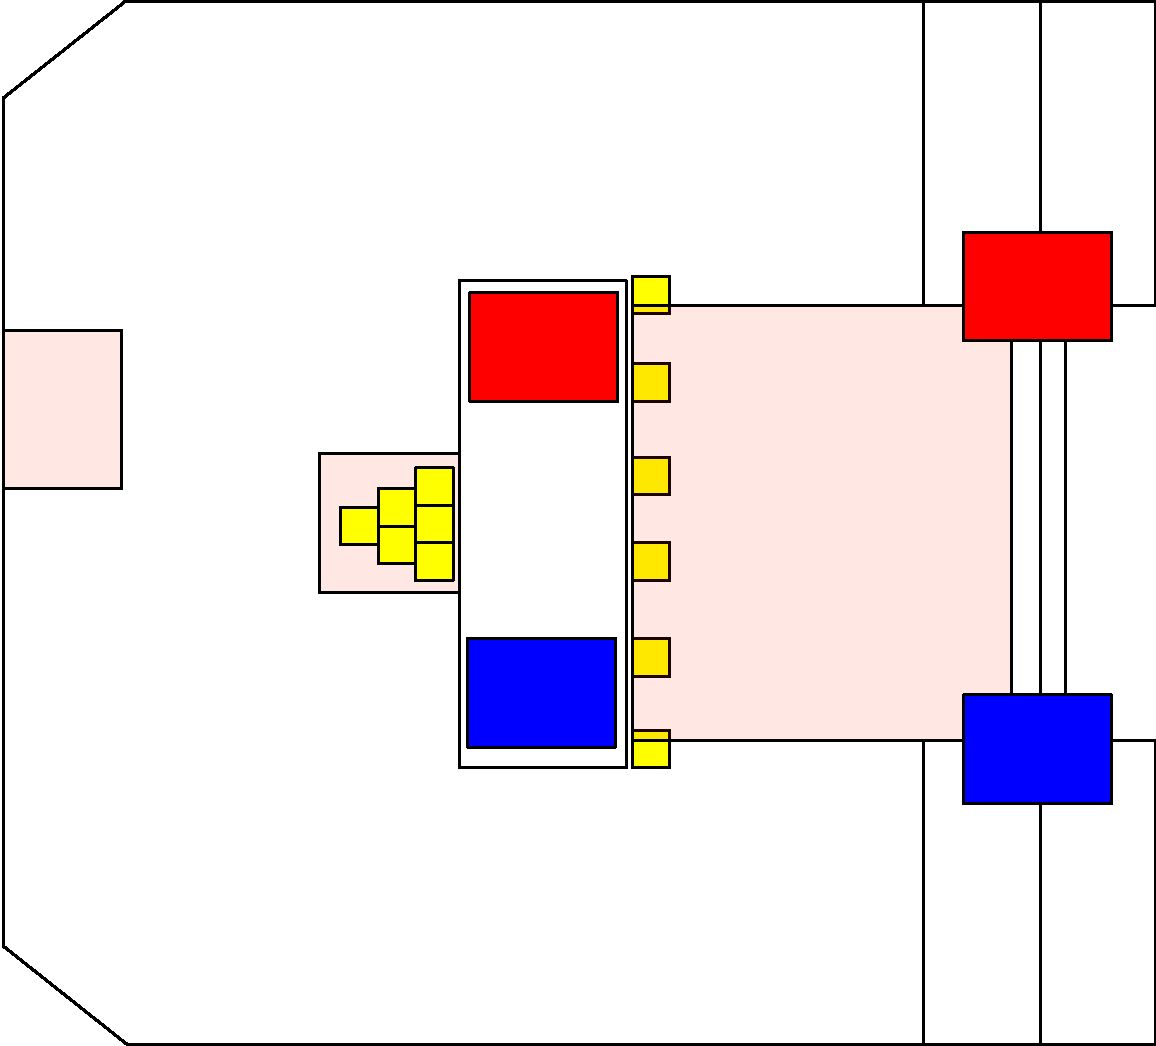
\includegraphics[scale=0.15]{assets/paths/BLANK_LL}
  \end{figure}
  \begin{figure}
   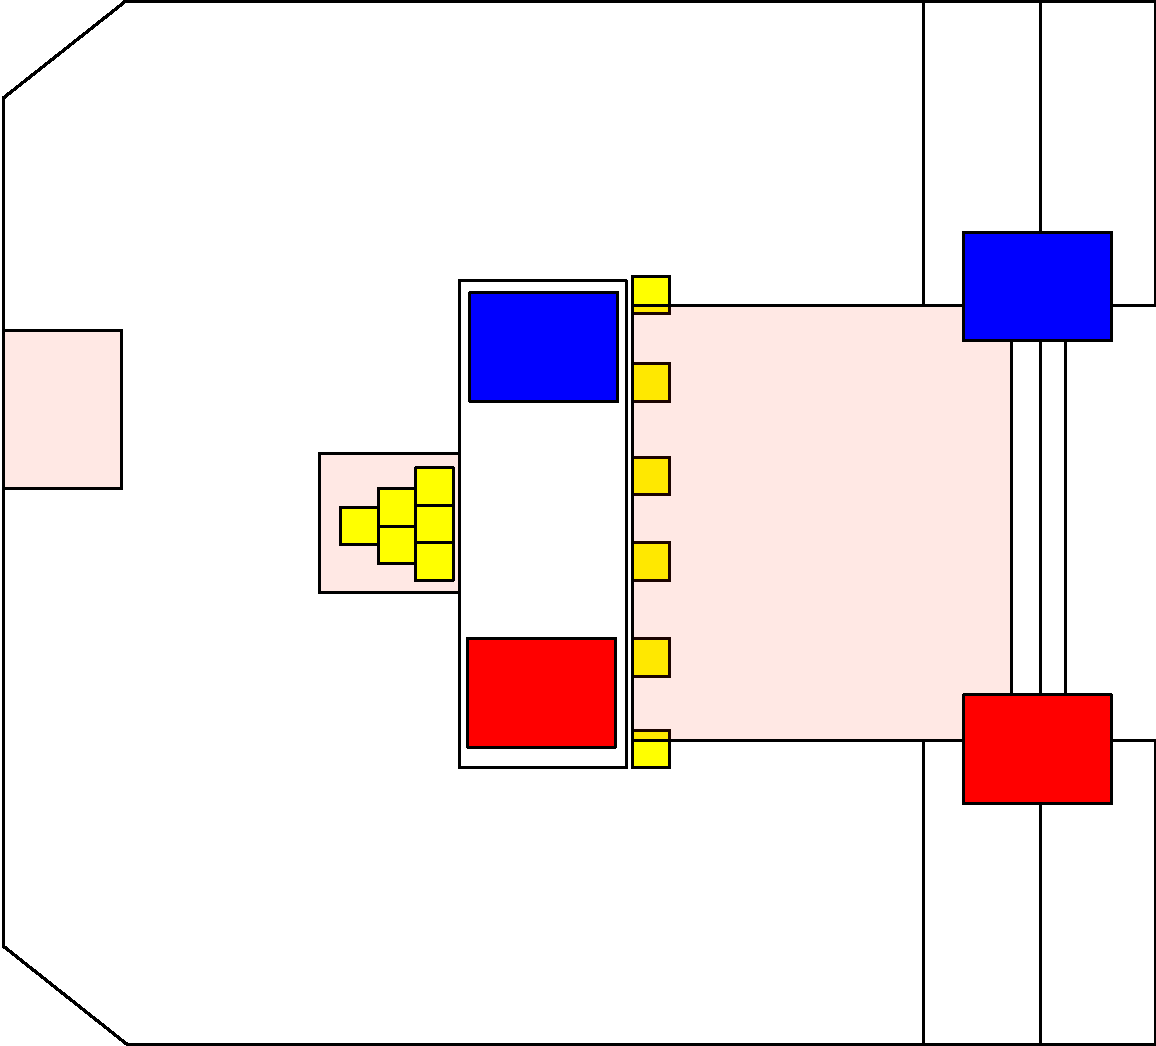
\includegraphics[scale=0.15]{assets/paths/BLANK_RR}
  \end{figure}
 \end{columns}
\end{frame}
%--- Next Frame ---%

\begin{frame}
  \center 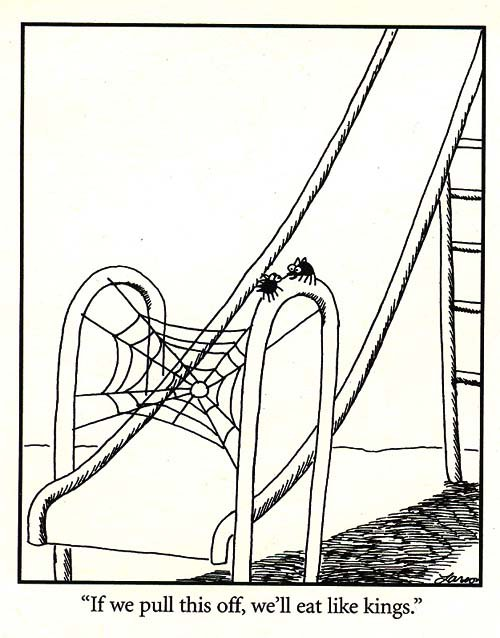
\includegraphics[scale=1.0]{assets/kings}
\end{frame}
%--- Next Frame ---%

\end{document}
